\section{Proof of the lower bound}
\label{app:lower-proof}

This section proves the finite matching lower bound in
\cref{app:thm:nonlinear-finite-lower} and states and proves its class
inclusion in \cref{app:prop:hard-family-inclusion}.
The matching proof allows randomized,
adaptive, value-dependent algorithms, interleaved counterfactual submissions,
and unrestricted returned bandwidth.  Only deterministic envelopes for the two pathwise counters in
\textcolor{red}{\cref{app:def:resources}} are bounded.
The next step toward \cref{main:thm:lower-envelope} is in
Appendix~\ref{app:benchmark-specializations}:
\cref{app:cor:signal-calibrated-finite-lower} gives the finite calibration,
immediately followed by the fixed-accuracy derivation in
\cref{app:cor:fixed-accuracy-main}.
\ifincludeexponents
Independent-signal rate results are in Appendix~\ref{app:independent-signal}.
\fi

\subsection{Proof overview}
\label{app:lower-proof-overview}

The goal is to show that few counterfactual submissions and few commit
rounds cannot both yield small sampling error.  We use a hidden perfect
matching: each position has one hidden trigger among \(\HardBankSize\)
candidates, and the oracle conceals an edge's dependence until a trigger
is hit.  The argument has three steps.

\paragraph{1. At most one candidate per source per submission.}
A state can return many rows but tests at most one candidate at each
source.  Conditional uniformity bounds the probability of hitting a given
source before retirement within \(\QueryBudget{}\) submissions by
\(\QueryBudget{}/\HardBankSize\). Summing over positions gives
\(\mathbb E\GenieDeletions\le N\QueryBudget{}/\HardBankSize\), where
\(\GenieDeletions\) counts query-retired edges.

\paragraph{2. Few commit rounds force collisions.}
Every edge not retired by a query must be retired at its first endpoint
commit.  Few rounds therefore require large active batches.  Conditional
uniformity makes such batches likely to contain both endpoints of an
unresolved edge: a \emph{collision}.  Edge counting and a conditional
Laplace bound give \(\TotalCollisions\gtrsim N/\RoundBudget{}\) collisions
with constant probability under the budget conditions of
\cref{app:thm:nonlinear-finite-lower}.

\paragraph{3. Collisions turn hidden dependence into sampling error.}
At a collision, sampling independently from the correct marginals
\(\HardMarginal\) misses the edge's dependence.  The one-edge squared
Hellinger loss \(\HardEdgeDistance\asymp\EdgeCoupling^2\) gives a local
affinity factor \(1-\HardEdgeDistance\).  The midpoint identity combines
these factors along adaptive paths to bound output error.
Here query-disclosure and collision probabilities use the
instance--midpoint law \eqref{app:eq:joint-instance-midpoint-law}, with
the decision-rule seed fixed; the final conclusion concerns the sampler's
seed-averaged TV risk.  The table locates the results that implement these
three steps.

\begin{table}[H]
\centering
\small
\begin{tabularx}{\linewidth}{@{}>{\raggedright\arraybackslash}p{0.23\linewidth}
  >{\raggedright\arraybackslash}X
  >{\raggedright\arraybackslash}p{0.23\linewidth}@{}}
\toprule
Proof step & Key idea and conclusion & References \\
\midrule
\textbf{Construct a hard matching family}
& Nontrigger oracle replies hide dependence while each edge retains
loss \(\HardEdgeDistance\asymp\EdgeCoupling^2\).  The inclusion calculation
checks the target assumptions and oracle error under the stated calibration.
&
\cref{app:lower-proof-family};
\cref{app:lem:hard-local-facts,app:prop:hard-family-inclusion} \\
\addlinespace
\textbf{Relate adaptive commits to output error}
& Later batches depend on sampled values.  The midpoint identity expresses
output affinity as an expectation of products of local affinities along
these adaptive paths.
&
\cref{app:lower-proof-midpoint};
\cref{app:lem:adaptive-midpoint-lower} \\
\addlinespace
\textbf{Limit what probes can reveal}
& The unresolved matching and triggers remain conditionally uniform.
One candidate per source per submission gives
\(\mathbb E\GenieDeletions\le N\QueryBudget{}/\HardBankSize\).
&
\cref{app:lower-proof-invariant};
\cref{app:lem:unresolved-invariant,app:lem:query-disclosure} \\
\addlinespace
\textbf{Force collisions with few rounds}
& Edge counting forces large active batches; a conditional Laplace bound
then gives \(\TotalCollisions\gtrsim N/\RoundBudget{}\) with constant
probability under the budgets in \eqref{app:eq:lower-proof-spine}.
&
\cref{app:lower-proof-collisions,app:lower-proof-matching-laplace,app:lower-proof-collision-tail};
\cref{app:lem:pathwise-edge-counting,app:lem:matching-collision-laplace,app:prop:collision-lower-tail} \\
\addlinespace
\textbf{Convert collisions into sampling error}
& Each collision contributes a factor \(1-\HardEdgeDistance\).
The midpoint identity gives a prior-averaged loss; averaging over seeds
and selecting a worst-case instance yields the TV lower bound.
&
\cref{app:lower-proof-affinity,app:lower-proof-nonlinear};
\cref{app:lem:collision-affinity,app:thm:nonlinear-finite-lower} \\
\addlinespace
\textbf{Recover the main-text lower bound}
& Calibrate the matching witness at the public parameters, then take the
fixed-accuracy limit to obtain \cref{main:thm:lower-envelope}.
&
\cref{app:cor:signal-calibrated-finite-lower,app:cor:fixed-accuracy-main} \\
\bottomrule
\end{tabularx}
\caption{Proof steps for the lower bound.}
\label{app:tab:lower-proof-map}
\end{table}

\ifincludeexponents
The joint-limit result in \cref{app:cor:benchmark-hellinger} and
independent-signal rates in \cref{app:lower-proof-rates} are also separate
extensions.
\fi

\paragraph{Quantitative summary.}
For every fixed decision-rule seed \(w\), the finite hypotheses and
constants give the following chain:
\begin{equation}
 \begin{aligned}
 &\QueryBudget{}\le\HardBankSize/8,\quad
 1\le\RoundBudget{}\le N/16384\\
 &\Longrightarrow\quad
 \mathbb E\GenieDeletions\le N/8\\
 &\Longrightarrow\quad
 \mathbb P\left(\TotalCollisions\ge
                 \frac{N}{8192\RoundBudget{}}\right)\ge\frac14\\
 &\Longrightarrow\quad
 \mathbb E_{I\sim\HardInstancePrior}\sqHellinger
   (\HardTargetLaw{I},\HardOutputLaw{I}{w})
 \ge\frac14\left[1-\exp\left\{
       -\frac{N\EdgeCoupling^2}{98304\RoundBudget{}}\right\}\right].
 \end{aligned}
 \label{app:eq:lower-proof-spine}
\end{equation}
The collision step combines the unresolved-matching invariant, the
edge-counting identity, and the conditional Laplace bound.
The last step uses the adaptive midpoint identity and
$\HardEdgeDistance\ge\EdgeCoupling^2/12$.

\subsection{Hard-family local facts and class membership}
\label{app:lower-proof-family}

This subsection proves the one-edge calculations in
\cref{app:lem:hard-local-facts}: positivity and common marginals, the edge
response, the selected-oracle error, and the one-edge Hellinger loss.  The
same calculations then verify \cref{app:prop:hard-family-inclusion}, placing
the finite hard family inside the shared target/oracle class used by both
bounds.

\paragraph{Intuition.}
There are two different error scales.  Removing one dependence edge costs
$\HardEdgeDistance\simeq\EdgeCoupling^2$, whereas replacing a nontrigger
conditional by the neutral marginal costs at most order
$\EdgeCoupling^2\TriggerMass$.  The extra factor $\TriggerMass$ lets the
frozen oracle hide failed trigger tests while preserving a larger loss
when two unresolved endpoints are committed together.

For the moment calculations, if
\(A\sim\HardMarginal\), then the trigger indicator at position \(i\) is
Bernoulli with mean \(\TriggerMass\).  Hence
\begin{equation}
 \mathbb E\TriggerFeature{i}(A)=0,
 \qquad
 \mathbb E\TriggerFeature{i}(A)^2=\TriggerVariance,
 \qquad
 \mathbb E|\TriggerFeature{i}(A)|=2\TriggerVariance.
 \label{app:eq:hard-feature-moments}
\end{equation}
Indeed, the feature is $1-\TriggerMass$ with probability $\TriggerMass$
and $-\TriggerMass$ otherwise, so
\[
\begin{aligned}
 \mathbb E\TriggerFeature{i}
 &=\TriggerMass(1-\TriggerMass)
   -(1-\TriggerMass)\TriggerMass=0,\\
 \mathbb E\TriggerFeature{i}^2
 &=\TriggerMass(1-\TriggerMass)^2
   +(1-\TriggerMass)\TriggerMass^2
   =\TriggerMass(1-\TriggerMass),\\
 \mathbb E|\TriggerFeature{i}|
 &=\TriggerMass(1-\TriggerMass)
   +(1-\TriggerMass)\TriggerMass
   =2\TriggerMass(1-\TriggerMass).
\end{aligned}
\]

\begin{lemma}[Local facts for the hard matching family]
\label{app:lem:hard-local-facts}
Under \eqref{app:eq:hard-basic-conditions}, every member of
\(\HardFamily[\HardVocabSize,\HardBankSize,
\TriggerMass,\EdgeCoupling]\) has the following properties.
\begin{enumerate}
 \item \textup{\textbf{Positivity, marginals, and factorization.}}
 Each edge law in \eqref{app:eq:hard-edge-law} is strictly positive,
 has both marginals equal to \(\HardMarginal\), and the product law satisfies
 the structural forest assumptions.
 \item \textup{\textbf{Edge response.}}
 For either orientation \(i\to j\) of a matching edge, the largest TV
 change in the endpoint kernel equals \(\EdgeCoupling\).
 \item \textup{\textbf{Oracle error.}}
 Let $j$ be any readout, let $i:=\MateInMatching{j}$, and let
 $a\in\Vocab\setminus\{\HardCandidate{\TriggerIndex{i}}\}$ be a revealed
 nontrigger value at $i$.  The selected oracle is exact outside this case,
 while in this case
 \begin{equation}
  \sqHellinger\bigl(
   \HardKernel{i}{j}{I}(\cdot\mid a),\HardMarginal
  \bigr)
  \le
  \frac{\EdgeCoupling^2\TriggerMass}
       {2(1-\TriggerMass)}
  \le \EdgeCoupling^2\TriggerMass.
  \label{app:eq:hard-local-oracle-error}
 \end{equation}
 \item \textup{\textbf{One-edge Hellinger loss.}}
 For every matching edge \(e\), uniformly over its two private trigger
 indices, the value below depends only on
 \((\TriggerMass,\EdgeCoupling)\), not on \(e\) or \(I\):
 \begin{equation}
  \frac{\EdgeCoupling^2}{12}
  \le
  \HardEdgeDistance
  :=\sqHellinger\bigl(
     \HardEdgeLaw{e}{I},\HardIndependentEdgeLaw{e}
    \bigr)
  \le\frac{\EdgeCoupling^2}{2}.
  \label{app:eq:hard-edge-distance}
 \end{equation}
\end{enumerate}
\end{lemma}

\begin{proof}

\emph{1. Positivity, common marginals, and forest factorization.}
Fix \(e=\{i,j\}\).  Summing \eqref{app:eq:hard-edge-law} over its second
coordinate and using \eqref{app:eq:hard-feature-moments} gives
\[
 \sum_b\HardEdgeLaw{e}{I}(a,b)
 =\HardMarginal(a)
  \left[1+
   \EdgeCoupling\frac{\TriggerFeature{i}(a)}{\TriggerVariance}
   \mathbb E\TriggerFeature{j}(B)
  \right]
 =\HardMarginal(a),
\]
where \(B\sim\HardMarginal\).  The other marginal follows symmetrically.
The likelihood ratio with respect to
\(\HardIndependentEdgeLaw{e}\) takes the three values
\begin{equation}
 1+\EdgeCoupling
   \frac{\TriggerFeature{i}(a)\TriggerFeature{j}(b)}
        {\TriggerVariance}
 =
 \begin{cases}
  1+\EdgeCoupling(1-\TriggerMass)/\TriggerMass,
    &a,b\text{ are their respective triggers},\\
  1-\EdgeCoupling,
    &\text{exactly one of }a,b\text{ is its trigger},\\
  1+\EdgeCoupling\TriggerMass/(1-\TriggerMass),
    &a,b\text{ are both nontriggers}.
 \end{cases}
 \label{app:eq:hard-likelihood-values}
\end{equation}
The conditions
\(0<\EdgeCoupling\le\TriggerMass\le1/2\) place every value in
\([1/2,2]\), proving strict positivity.  The marginal identity also gives
the endpoint compatibility
\[
 \HardMarginal(a)\HardKernel{i}{j}{I}(b\mid a)
 =\HardEdgeLaw{e}{I}(a,b)
 =\HardMarginal(b)\HardKernel{j}{i}{I}(a\mid b).
\]
Every component is one edge, so multiplying these identities over the hidden
matching proves the required forest factorization for either root choice.


\emph{2. Directed endpoint response.}
For source values \(a,a'\),
\begin{align}
 &\dTV\bigl(
   \HardKernel{i}{j}{I}(\cdot\mid a),
   \HardKernel{i}{j}{I}(\cdot\mid a')
  \bigr)\notag\\
 &\qquad=
 \frac{\EdgeCoupling
       |\TriggerFeature{i}(a)-\TriggerFeature{i}(a')|}
      {2\TriggerVariance}
 \sum_b\HardMarginal(b)|\TriggerFeature{j}(b)|
 =\EdgeCoupling
  |\TriggerFeature{i}(a)-\TriggerFeature{i}(a')|.
 \label{app:eq:hard-directed-response}
\end{align}
The feature equals \(1-\TriggerMass\) at the unique trigger and
\(-\TriggerMass\) elsewhere.  Its largest difference is therefore one, so
the maximum in \eqref{app:eq:hard-directed-response} is exactly
\(\EdgeCoupling\).


\emph{3. Oracle error at a revealed nontrigger.}
Because the target is a product over matching edges, the exact row at a
readout \(j\) is \(\HardMarginal\) when its mate is masked and is
\(\HardKernel{i}{j}{I}(\cdot\mid y_i)\) when the mate \(i\) is revealed.
Thus \eqref{app:eq:hard-oracle} is exact in its first two cases.  In the third
case, $\TriggerFeature{i}(y_i)=-\TriggerMass$, so the likelihood ratio is
\[
 \frac{\HardKernel{i}{j}{I}(b\mid y_i)}{\HardMarginal(b)}
 =1-\frac{\EdgeCoupling}{1-\TriggerMass}\TriggerFeature{j}(b).
\]
Substitution into the definition of chi-square divergence gives
\begin{align}
 \ChiSquareDivergence{
  \HardKernel{i}{j}{I}(\cdot\mid y_i)}{\HardMarginal}
 &=\sum_b\HardMarginal(b)
       \left(\frac{\EdgeCoupling\TriggerFeature{j}(b)}
                   {1-\TriggerMass}\right)^2\notag\\
 &=\frac{\EdgeCoupling^2}{(1-\TriggerMass)^2}
       \TriggerMass(1-\TriggerMass)
 =\EdgeCoupling^2\frac{\TriggerMass}{1-\TriggerMass}.
 \label{app:eq:hard-oracle-chi-square}
\end{align}
For a likelihood ratio \(r\),
\((\sqrt r-1)^2\le(r-1)^2\).  The normalization in
\eqref{app:eq:distances} therefore implies
\(\sqHellinger(p,q)\le\ChiSquareDivergence{p}{q}/2\).  Combining this with
\eqref{app:eq:hard-oracle-chi-square} and
\(\TriggerMass\le1/2\) proves \eqref{app:eq:hard-local-oracle-error}.


\emph{4. One-edge squared-Hellinger loss.}
Finally, put
\[
 Z_e(a,b):=
 \frac{\TriggerFeature{i}(a)\TriggerFeature{j}(b)}
      {\TriggerVariance}.
\]
Under \(\HardIndependentEdgeLaw{e}\), each endpoint independently equals
its trigger token with probability \(\TriggerMass\).  Thus
\[
 Z_e=
 \begin{cases}
 (1-\TriggerMass)/\TriggerMass,
   &\text{with probability }\TriggerMass^2
      \quad\text{(both triggers)},\\
 -1,
   &\text{with probability }2\TriggerMass(1-\TriggerMass)
      \quad\text{(one trigger)},\\
 \TriggerMass/(1-\TriggerMass),
   &\text{with probability }(1-\TriggerMass)^2
      \quad\text{(neither trigger)}.
 \end{cases}
 \]
This law depends only on \(\TriggerMass\), not on the edge or its trigger
indices.
\Eqref{app:eq:hard-feature-moments} and independence under
\(\HardIndependentEdgeLaw{e}\) give
\[
 \mathbb E_{\HardIndependentEdgeLaw{e}}Z_e
 =\frac{\mathbb E\TriggerFeature{i}\,
        \mathbb E\TriggerFeature{j}}{\TriggerVariance}=0,\qquad
 \mathbb E_{\HardIndependentEdgeLaw{e}}Z_e^2
 =\frac{\mathbb E\TriggerFeature{i}^2\,
        \mathbb E\TriggerFeature{j}^2}{(\TriggerVariance)^2}=1.
\]  Since
\(\mathrm d\HardEdgeLaw{e}{I}/\mathrm d\HardIndependentEdgeLaw{e}
=1+\EdgeCoupling Z_e\),
the definition of squared Hellinger distance gives the first line below.
For the second, multiply
$\sqrt{1+\EdgeCoupling Z_e}-1$ by
$(\sqrt{1+\EdgeCoupling Z_e}+1)/
 (\sqrt{1+\EdgeCoupling Z_e}+1)$:
\begin{align}
 \HardEdgeDistance
 &=\frac12\mathbb E_{\HardIndependentEdgeLaw{e}}
       \bigl(\sqrt{1+\EdgeCoupling Z_e}-1\bigr)^2\notag\\
 &=\frac{\EdgeCoupling^2}{2}
  \mathbb E_{\HardIndependentEdgeLaw{e}}
  \frac{Z_e^2}
       {(\sqrt{1+\EdgeCoupling Z_e}+1)^2}.
 \label{app:eq:hard-edge-distance-formula}
\end{align}
Consequently \(\HardEdgeDistance\) depends only on
\((\TriggerMass,\EdgeCoupling)\), so it is the same for every matching
component and every choice of its trigger indices.
By \eqref{app:eq:hard-likelihood-values}, the denominator lies between
one and \((\sqrt2+1)^2<6\).
\Eqref{app:eq:hard-edge-distance} follows.
\end{proof}

\paragraph{Intuition for class inclusion.}
The four checks have separate jobs:
$\HardVocabSize\TriggerMass>1$ puts the candidate bank above the background,
$\TriggerMass\le\HardBankSize^{-\RankTailExponent}$ gives the frequency
envelope, $\EdgeSignal\le\EdgeCoupling$ gives the edge signal, and
$\EdgeCoupling^2\TriggerMass\le(\OracleRadius)^2/(2N)$ hides nontrigger replies
within the oracle budget.  In the main calibration,
$\EdgeCoupling=\TriggerMass=\EdgeSignal$, so the last check becomes the
cubic constraint $\EdgeSignal^3\le(\OracleRadius)^2/(2N)$.

\begin{proposition}[Finite hard-family inclusion]
\label{app:prop:hard-family-inclusion}
In addition to \eqref{app:eq:hard-basic-conditions}, let
$\RankTailExponent>1$, use the same public vocabulary of size $\VocabSize$,
set
$\ResponseExponent=\ResponseConstant=\FrequencyConstant=1$, and suppose
\begin{equation}
 \HardVocabSize\TriggerMass>1,
 \qquad
 \TriggerMass\le\HardBankSize^{-\RankTailExponent},
 \qquad
 \EdgeSignal\le\EdgeCoupling,
 \qquad
 \EdgeCoupling^2\TriggerMass\le\frac{(\OracleRadius)^2}{2N}.
 \label{app:eq:finite-hard-inclusion}
\end{equation}
Then every target in
$\HardFamily[\HardVocabSize,\HardBankSize,\TriggerMass,\EdgeCoupling]$
satisfies the structural and response assumptions in
Appendix~\ref{app:setup}, as well as the finite rank--frequency inequality in
(RF\textcolor{red}{; \cref{app:eq:RF}}), and its selected oracle \eqref{app:eq:hard-oracle} belongs to
$\OracleClass(\HardTargetLaw{I};\OracleRadius)$.  If the public vocabulary
sequence also obeys the vocabulary-growth condition in (RF\textcolor{red}{; \cref{app:ass:rate-regime}}), then the full
(RF\textcolor{red}{; \cref{app:ass:rate-regime}}) assumption holds.  Under that additional asymptotic condition, this
matching family is a contained subfamily of the same public problem class
used by the upper theorem.
\end{proposition}

\begin{proof}[Proof of \cref{app:prop:hard-family-inclusion}]

\emph{1. Forest structure and the edge-signal condition (UEN\textcolor{red}{; \cref{app:eq:UEN}}).}
Apply \cref{app:lem:hard-local-facts}.  Its first conclusion proves
strict positivity and Assumption~\ref{app:ass:forest-structure}.  Complete
boundary assignments outside a matching edge do not alter that edge's law,
so \eqref{app:eq:hard-directed-response} makes both directed intrinsic
responses exactly \(\EdgeCoupling\).  The condition
\(\EdgeSignal\le\EdgeCoupling\) therefore proves (UEN\textcolor{red}{; \cref{app:eq:UEN}}).


\emph{2. Response-tail regularity (RT\textcolor{red}{; \cref{app:eq:RT}}).}
For (RT\textcolor{red}{; \cref{app:eq:RT}}), first consider distinct positions \(i,j\) that are not matched.
Conditioning on a complete boundary fixes the mates of \(i\) and \(j\), and
the product over matching components makes
\(\BoundaryRow{i}{j}{a}{z}\) independent of \(a\).  The response diameter is
therefore zero.

It remains to consider a matching edge.  Fix a threshold
\(t\).
\begin{itemize}
\item If \(t<\TriggerMass\), the marginal tail
contains no candidate token and hence no trigger.  Every source value in the
tail has the same centered feature \(-\TriggerMass\), so its response
diameter is zero.
\item If \(t\ge\TriggerMass\), the response diameter is at most
\(\EdgeCoupling\le\TriggerMass\le t\).
\end{itemize}
Thus (RT\textcolor{red}{; \cref{app:eq:RT}}) holds with
\(\ResponseExponent=\ResponseConstant=1\).


\emph{3. Rank--frequency regularity (RF\textcolor{red}{; \cref{app:eq:RF}}).}
The inequality \(\HardVocabSize\TriggerMass>1\) is equivalent to the
background mass in \eqref{app:eq:hard-common-marginal} being strictly less
than $\HardVocabSize^{-1}$, since
\[
 \frac{1-\HardBankSize\TriggerMass}{\HardVocabSize-\HardBankSize}
 <\frac1{\HardVocabSize}
 \quad\Longleftrightarrow\quad
 \HardVocabSize-\HardVocabSize\HardBankSize\TriggerMass
 <\HardVocabSize-\HardBankSize
 \quad\Longleftrightarrow\quad
 \HardVocabSize\TriggerMass>1.
\]  Hence the \(\HardBankSize\) candidates occupy
the first \(\HardBankSize\) marginal ranks.  For
\(k\le\HardBankSize\),
\[
 \HardMarginal(\HardCandidate{k})=\TriggerMass
 \le\HardBankSize^{-\RankTailExponent}
 \le k^{-\RankTailExponent};
\]
for \(k>\HardBankSize\), the vocabulary-floor term
\(\HardVocabSize^{-1}\) suffices.  This proves the rank--frequency inequality
in (RF\textcolor{red}{; \cref{app:eq:RF}}) with \(\FrequencyConstant=1\).  The separate vocabulary-growth clause
in (RF\textcolor{red}{; \cref{app:ass:rate-regime}}) holds whenever the public sequence \(\HardVocabSize\) has the
declared asymptotic scaling.


\emph{4. Uniform oracle accuracy (A2).}
The only nonzero oracle error is bounded by
\eqref{app:eq:hard-local-oracle-error}.  The final condition in
\eqref{app:eq:finite-hard-inclusion} therefore places it below
\((\OracleRadius)^2/(2N)\), proving (A2).  All required finite conditions hold
for every hidden matching and trigger vector.  Together with the stated
vocabulary-growth condition, this proves the asserted inclusion in the
shared asymptotic class.
\end{proof}

% Please keep the comparison's goal, obstacle, and bridge on the same page.
\begin{samepage}
\subsection{Adaptive midpoint comparison and instance prior}
\label{app:lower-proof-midpoint}

We relate the target law to the sampler's output law through the discrepancies
at individual commits. Three points guide the comparison:
\begin{itemize}
\item \emph{Goal.} Express the output affinity, or equivalently one minus the
squared-Hellinger error, in terms of local commit affinities.
\item \emph{Obstacle.} A different committed value can change subsequent
probes, batches, and the stopping round. Thus local affinities depend on the
realized history; the fixed-product affinity formula does not directly
combine them.
\item \emph{Bridge.} Normalize the geometric mean of the two commit kernels
at each history. These normalized kernels define a common path law under
which the product of local affinities equals the output affinity in
expectation (\cref{app:lem:adaptive-midpoint-lower}).
\end{itemize}
\end{samepage}

\emph{Fixed objects.}
Fix an admissible algorithm with finite pathwise budgets
\((\QueryBudget{},\RoundBudget{})\), an instance
\(I=(\HiddenMatching,\TriggerVector)\) of
\cref{app:def:hard-matching-family}, and one value \(w\) of the
decision-rule seed. Put
\begin{equation}
 \HardOutputLaw{I}{w}
 :=\SamplerOutputLaw{w}{\HardOracle{I}}.
 \label{app:eq:hard-seeded-output-law}
\end{equation}
The following three executions differ in their commit kernels, defined
below. The exact comparison process has terminal law \(\HardTargetLaw{I}\);
Step~2 of the proof verifies this even for adaptive batches.

\begin{center}
\small
\begin{tabularx}{\linewidth}{@{}>{\raggedright\arraybackslash}p{0.23\linewidth}
  >{\raggedright\arraybackslash}p{0.32\linewidth}
  >{\raggedright\arraybackslash}X@{}}
\toprule
Execution & Commit kernel at history \(h\) & Law and role \\
\midrule
Exact comparison
& \(\HardExactBatchLaw{t}{I}(\cdot\mid h)\): true joint conditional
& \(\HardTargetLaw{I}\): target output law. \\
\addlinespace
Product-commit sampler
& \(\HardProductBatchLaw{t}{I}(\cdot\mid h)\): product of oracle rows
& \(\HardOutputLaw{I}{w}\): output law being evaluated. \\
\addlinespace
Adaptive midpoint
& \(\HardMidpointKernel{t}{I}(\cdot\mid h)\): normalized geometric mean
& \(\HardMidpointLaw{I}{w}\): analytic path law for averaging local affinities. \\
\bottomrule
\end{tabularx}
\end{center}

\begin{itemize}
\item \emph{Shared operations.} All three use the same seed-fixed decision
rule and the same frozen oracle \(\HardOracle{I}\) for probes. At a common
history they select the same batch \(B_t(h)\).
\item \emph{Changed operation.} Only the law of the committed values changes.
The resulting histories, and hence later batches, can differ between executions.
\end{itemize}

\begin{definition*}[Commit kernels and adaptive midpoint law]
\emph{History and batch.}
Immediately before commit \(t\), after the intervening probes, let \(h\)
be the complete observable history: committed positions and values,
the earlier oracle transcript, and the decision-rule state.
Thus $h=\OpVisibleHistory{s_t}$ in the operation notation of
\cref{app:eq:operation-action,app:eq:operation-visible-history}.
Write \(G(h)\) for the committed set, \(x_{G(h)}\) for its values, and
\(y_t(h)\) for the commit state in \eqref{app:eq:commit-state}.
For fixed \((I,w)\), the probes and batch selection are deterministic
functions of the observed past; write \(B_t(h)\) for the selected batch.
The seed \(w\) is suppressed from local kernels because \(h\) includes
the seed-fixed decision-rule state, but retained in full-law and
terminal-round notation.

\emph{Commit kernels.}
For \(z\in\Vocab^{B_t(h)}\), define
\begin{align}
 \HardExactBatchLaw{t}{I}(z\mid h)
 &:=\HardTargetLaw{I}\bigl(
   X_{B_t(h)}=z\mid X_{G(h)}=x_{G(h)}
  \bigr),
 \label{app:eq:hard-exact-batch-law}\\
 \HardProductBatchLaw{t}{I}(z\mid h)
 &:=\prod_{j\in B_t(h)}\HardOracleRowMass{I}{y_t(h)}{j}{z_j}.
 \label{app:eq:hard-product-batch-law}
\end{align}

\emph{Local affinity and midpoint law.}
Define
\begin{align}
 \HardLocalAffinity{t}{I,h}
 &:=\sum_{z\in\Vocab^{B_t(h)}}
    \sqrt{
     \HardExactBatchLaw{t}{I}(z\mid h)
     \HardProductBatchLaw{t}{I}(z\mid h)},
 \label{app:eq:hard-local-affinity}\\
 \HardMidpointKernel{t}{I}(z\mid h)
 &:=\frac{
    \sqrt{
     \HardExactBatchLaw{t}{I}(z\mid h)
     \HardProductBatchLaw{t}{I}(z\mid h)}}
   {\HardLocalAffinity{t}{I,h}}.
 \label{app:eq:hard-midpoint-kernel}
\end{align}
Let \(\HardMidpointLaw{I}{w}\) be the analytic adaptive path law that runs
the same decision rule and frozen-oracle probes, drawing every commit
batch from \(\HardMidpointKernel{t}{I}(\cdot\mid h)\).
\end{definition*}

\paragraph{Why the construction is well defined.}
\begin{itemize}
\item \emph{Conditioning on the history.}
For fixed \((I,w)\), every reachable \(h\) can be reconstructed from
\(x_{G(h)}\): replay the seed-fixed decision rule from the initial state and,
at each earlier commit, supply the coordinates of \(x_{G(h)}\) selected
by that commit. The frozen oracle reproduces the intervening replies,
batches, and decision-rule states. Conversely, \(h\) records \(x_{G(h)}\).
Thus conditioning on this \(h\) adds no random event beyond
\(X_{G(h)}=x_{G(h)}\), justifying
\eqref{app:eq:hard-exact-batch-law}.
\item \emph{Normalization.}
Strict positivity makes the denominator nonzero. Cauchy--Schwarz gives
\(0<\HardLocalAffinity{t}{I,h}\le1\). In particular,
\[
 \sum_{z\in\Vocab^{B_t(h)}}\HardMidpointKernel{t}{I}(z\mid h)
 =\frac{\displaystyle
   \sum_{z\in\Vocab^{B_t(h)}}
    \sqrt{\HardExactBatchLaw{t}{I}(z\mid h)
           \HardProductBatchLaw{t}{I}(z\mid h)}}
  {\HardLocalAffinity{t}{I,h}}
 =\frac{\HardLocalAffinity{t}{I,h}}{\HardLocalAffinity{t}{I,h}}
 =1.
\]
\item \emph{Pathwise budgets.}
Both commit kernels are strictly positive, so the midpoint kernel has
the same support at every reachable history. It therefore traverses the
same decision tree as the implemented sampler. Every midpoint path has
at most \(\QueryBudget{}\) counterfactual submissions and at most
\(\RoundBudget{}\) nonempty commits.
\end{itemize}

\paragraph{From local affinity to output error.}
The defining factorization is
\[
 \sqrt{\HardExactBatchLaw{t}{I}(z\mid h)
        \HardProductBatchLaw{t}{I}(z\mid h)}
 =\HardLocalAffinity{t}{I,h}\HardMidpointKernel{t}{I}(z\mid h).
\]
Along a complete path, the normalized \(\HardMidpointKernel{t}{I}\) factors
supply its midpoint probability, while the \(\HardLocalAffinity{t}{I,h}\)
factors retain the local affinity losses.
The next identity averages their product over the adaptive paths.

\begin{lemma}[Adaptive midpoint identity]
\label{app:lem:adaptive-midpoint-lower}
For every fixed instance \(I\) and decision-rule seed \(w\),
\begin{equation}
 1-\sqHellinger(
      \HardTargetLaw{I},\HardOutputLaw{I}{w})
 =\mathbb E_{H\sim\HardMidpointLaw{I}{w}}
   \prod_{t=1}^{\HardTerminalRoundCount{I}{w}{H}}
    \HardLocalAffinity{t}{I,H_{t-1}},
 \label{app:eq:adaptive-midpoint-identity}
\end{equation}
where \(\HardTerminalRoundCount{I}{w}{H}\le \RoundBudget{}\) is the terminal number of
nonempty commit batches on the midpoint path.
Here \(H_{t-1}\) denotes the complete observable history immediately
before commit \(t\), after all intervening counterfactual operations.
The subscript counts earlier commits, not individual query operations.
\end{lemma}

The remaining lower-bound argument uses this identity at two levels:
\begin{itemize}
\item \emph{Local penalty.} \Cref{app:lem:collision-affinity} bounds the
factors \(\HardLocalAffinity{t}{I,h}\) using unresolved edges whose
endpoints are committed together.
\item \emph{Global error.} The survivor and collision arguments count
these events under the instance--midpoint law
\eqref{app:eq:joint-instance-midpoint-law}. The identity converts that
count into an output-error bound.
\end{itemize}

\begin{proof}

\emph{1. Reconstruct the unique adaptive path.}
Fix a complete output \(x\in\Vocab^N\).  Starting with the empty history,
replay the deterministic seed-fixed decision rule.  Whenever it chooses
\(B_t(h_{t-1}(x))\), feed it
\(z_t(x):=x_{B_t(h_{t-1}(x))}\).  This recursively determines the histories,
batches, and terminal round \(\HardTerminalRoundCount{I}{w}{x}\).  No
remasking makes the realized batches disjoint and exhaustive.  Put
\(G_t(x):=G_{t-1}(x)\cup B_t(h_{t-1}(x))\), with \(G_0(x)=\varnothing\).

\emph{2. Factor the exact and product output masses.}
The exact conditional factors telescope:
\begin{align*}
 &\prod_{t=1}^{\HardTerminalRoundCount{I}{w}{x}}
   \HardExactBatchLaw{t}{I}(z_t(x)\mid h_{t-1}(x))\\
 &\quad=\prod_{t=1}^{\HardTerminalRoundCount{I}{w}{x}}
   \frac{\HardTargetLaw{I}(X_{G_t(x)}=x_{G_t(x)})}
        {\HardTargetLaw{I}(X_{G_{t-1}(x)}=x_{G_{t-1}(x)})}
 =\frac{\HardTargetLaw{I}(X_{\PositionSet}=x)}{1}
 =\HardTargetLaw{I}(x).
\end{align*}
Here the numerator at round \(t\) is the denominator at round \(t+1\);
the initial event has probability one and the terminal set is \(\PositionSet\).
This identity and the
product-commit rule therefore give
\begin{align}
 \HardTargetLaw{I}(x)
 &=\prod_{t=1}^{\HardTerminalRoundCount{I}{w}{x}}
   \HardExactBatchLaw{t}{I}
    (z_t(x)\mid h_{t-1}(x)),
 \label{app:eq:hard-exact-path-factorization}\\
 \HardOutputLaw{I}{w}(x)
 &=\prod_{t=1}^{\HardTerminalRoundCount{I}{w}{x}}
   \HardProductBatchLaw{t}{I}
    (z_t(x)\mid h_{t-1}(x)).
 \label{app:eq:hard-product-path-factorization}
\end{align}
The batch-selection rule has no likelihood factor because it is deterministic
given the displayed history.


\emph{3. Normalize the midpoint path mass.}
For the same terminal output, the midpoint path mass is
\begin{equation}
 \HardMidpointLaw{I}{w}(x)
 :=\prod_{t=1}^{\HardTerminalRoundCount{I}{w}{x}}
   \HardMidpointKernel{t}{I}
    (z_t(x)\mid h_{t-1}(x)).
 \label{app:eq:hard-midpoint-path-mass}
\end{equation}
To verify that this path mass sums to one, first account for paths that
finish at different rounds.  Nonempty batches are disjoint, so every path
has at most \(N\) rounds.  For this calculation only, pad each finished path
to \(N\) rounds by setting \(B_t(h)=\varnothing\),
\(\Vocab^\varnothing=\{\varnothing\}\), and
\(\HardMidpointKernel{t}{I}(\varnothing\mid h)=1\) after termination.
These extra factors leave \eqref{app:eq:hard-midpoint-path-mass} unchanged.
Each complete output corresponds to exactly one padded path, and conversely,
because the seed-fixed decision rule is deterministic and the genuine batches
are disjoint and exhaustive.

Write \(h_{t-1}\) for the history determined by the preceding assignments
\(z_1,\ldots,z_{t-1}\).  For any \(1\le r\le N\), hold
\(z_1,\ldots,z_{r-1}\) fixed.  The earlier factors do not depend on \(z_r\),
so the local normalization above gives
\begin{align*}
 &\sum_{z_r\in\Vocab^{B_r(h_{r-1})}}
   \prod_{t=1}^{r}\HardMidpointKernel{t}{I}(z_t\mid h_{t-1})\\
 &\quad=
   \left[\prod_{t=1}^{r-1}
     \HardMidpointKernel{t}{I}(z_t\mid h_{t-1})\right]
   \underbrace{\sum_{z_r\in\Vocab^{B_r(h_{r-1})}}
     \HardMidpointKernel{r}{I}(z_r\mid h_{r-1})}_{=1}\\
 &\quad=\prod_{t=1}^{r-1}
     \HardMidpointKernel{t}{I}(z_t\mid h_{t-1}).
\end{align*}
Applying this equality for \(r=N,N-1,\ldots,1\) removes the nested sums
from the innermost one outwards and ends with the empty product \(1\):
\[
 \sum_{x\in\Vocab^N}\HardMidpointLaw{I}{w}(x)
 =\sum_{z_1\in\Vocab^{B_1(h_0)}}\cdots
  \sum_{z_N\in\Vocab^{B_N(h_{N-1})}}
   \prod_{t=1}^{N}\HardMidpointKernel{t}{I}(z_t\mid h_{t-1})
 =1.
\]

\emph{4. Convert the affinity sum into a midpoint expectation.}
Substituting
\(\sqrt{\HardExactBatchLaw{t}{I}\HardProductBatchLaw{t}{I}}
 =\HardLocalAffinity{t}{I,h}\HardMidpointKernel{t}{I}\) into the terminal
affinity sum yields
\begin{align*}
 &\HellingerAffinity(
    \HardTargetLaw{I},\HardOutputLaw{I}{w})\\
 &\quad=\sum_{x\in\Vocab^N}
  \sqrt{\HardTargetLaw{I}(x)\HardOutputLaw{I}{w}(x)}\\
 &\quad=\sum_{x\in\Vocab^N}
  \HardMidpointLaw{I}{w}(x)
  \prod_{t=1}^{\HardTerminalRoundCount{I}{w}{x}}
   \HardLocalAffinity{t}{I,h_{t-1}(x)}\\
 &\quad=\mathbb E_{H\sim\HardMidpointLaw{I}{w}}
  \prod_{t=1}^{\HardTerminalRoundCount{I}{w}{H}}
   \HardLocalAffinity{t}{I,H_{t-1}}.
\end{align*}
Since \(\HellingerAffinity(p,q)=1-\sqHellinger(p,q)\), this is
\eqref{app:eq:adaptive-midpoint-identity}.
\end{proof}

\paragraph{Instance prior for the remaining proof.}
Keep the seed \(w\) fixed. Draw an instance
\(I=(\HiddenMatching,\TriggerVector)\) from the prior
\(\HardInstancePrior\) as follows:
\begin{itemize}
\item \emph{Matching.} \(\HiddenMatching\) is uniform over all perfect
matchings of \(\PositionSet\).
\item \emph{Triggers.} \(\TriggerIndex{1},\ldots,\TriggerIndex{N}\) are
independent uniform elements of \([\HardBankSize]\), independent of
\(\HiddenMatching\).
\end{itemize}
All random variables used in the remaining proof are evaluated under the
joint analytic law
\begin{equation}
 I\sim\HardInstancePrior,
 \qquad
 H\mid(I,w)\sim\HardMidpointLaw{I}{w}.
 \label{app:eq:joint-instance-midpoint-law}
\end{equation}

\subsection{Unresolved edges, survivor invariant, and query retirement}
\label{app:lower-proof-invariant}

We need two facts under the instance--midpoint law
\eqref{app:eq:joint-instance-midpoint-law}:
\begin{itemize}
\item \emph{The distribution left unresolved.}
\Cref{app:lem:unresolved-invariant} shows that the remaining matching is
uniform and its triggers are independent uniform remaining candidates.
This permits the conditional collision calculation below.
\item \emph{The number of query retirements.}
\Cref{app:lem:query-disclosure} bounds
\(\mathbb E\GenieDeletions\le N\QueryBudget{}/\HardBankSize\).
A submission tests at most one candidate at each source, so probes can
retire only a limited number of edges before commits touch them.
\end{itemize}
We first define retirement and the information used to condition these
two statements. The decision-rule seed \(w\) remains fixed.
Use the operation clock, actions \(A_s\), and visible histories
\(\OpVisibleHistory{s}\) from
\cref{app:eq:operation-action,app:eq:operation-visible-history}.
For a query, write \(y=\OpSubmittedState{s}\) and \(J=J_s\).
At commit \(t\), \(s=s_t\) and the batch is \(B_t=B_{t_s}\).

\begin{definition*}[Unresolved edges and the analytic record]
\emph{The test at one source.}
For any submitted state \(y\) and position \(i\in\PositionSet\), put
\begin{equation}
 \HardTest{y}{i}:=
 \begin{cases}
  c,&y_i=\HardCandidate{c}\text{ for some }c\in[\HardBankSize],\\
  \bot,&y_i=\MASK\text{ or }y_i\in\HardBackground,
 \end{cases}
 \qquad
 \HardHit{y}{i}:=
 \mathbf 1\{\HardTest{y}{i}=\TriggerIndex{i}\}.
 \label{app:eq:hard-test-and-hit}
\end{equation}
Thus \(y_i=\HardCandidate{c}\) tests the equality
\(\TriggerIndex{i}=c\). A mask or background value tests no candidate.

\emph{Unresolved edges and vertices.}
Let \(\OpUnresolvedMatching{s}\) be the edges unresolved immediately
before operation \(s\). Initialize \(\OpUnresolvedMatching{1}:=\HiddenMatching\)
and update by
\begin{equation}
 \OpUnresolvedMatching{s+1}:=
 \begin{cases}
  \{e\in\OpUnresolvedMatching{s}:
       \sum_{i\in e}\HardHit{y}{i}=0\},
       &\text{query of }y,\\
  \{e\in\OpUnresolvedMatching{s}:e\cap B_t=\varnothing\},
       &\text{commit }t.
 \end{cases}
 \label{app:eq:unresolved-matching-update}
\end{equation}
Define the unresolved vertex set by
\begin{equation}
 \OpUnresolvedVertices{s}:=\bigcup_{e\in\OpUnresolvedMatching{s}}e.
 \label{app:eq:unresolved-vertices}
\end{equation}
Thus a query retires an edge when at least one endpoint hits; a commit
retires it when \(e\cap B_t\ne\varnothing\). In either case both endpoints
leave \(\OpUnresolvedVertices{s}\). A query commits neither endpoint,
and a commit fixes only those in \(e\cap B_t\).
Because each update removes whole edges, \(\OpUnresolvedMatching{s}\)
is a perfect matching on \(\OpUnresolvedVertices{s}\).
The target law remains
\(\HardTargetLaw{I}(x)=\prod_{e\in\HiddenMatching}\HardEdgeLaw{e}{I}(x_e)\),
and the frozen oracle \(\HardOracle{I}\) remains unchanged.
In particular, an uncommitted vertex may lie on a retired edge.

\emph{Retirement record.}
For each newly retired edge, record its identity and both trigger indices:
\begin{equation}
 \OpRetiredRecord{s}:=
 \left\{\bigl(e,(\TriggerIndex{i})_{i\in e}\bigr):
 e\in\OpUnresolvedMatching{s}\setminus\OpUnresolvedMatching{s+1}\right\}.
 \label{app:eq:retirement-record}
\end{equation}
Endpoint tuples use the public position order. Let
\(\GenieDeletions:=\sum_{s:\,A_s\text{ is a query}}
 |\OpUnresolvedMatching{s}\setminus\OpUnresolvedMatching{s+1}|\).
Simultaneous hits on both endpoints count as one retired edge.

\emph{Remaining candidates.}
Initially \(\OpRemainingTriggers{i}{1}:=[\HardBankSize]\).
For each surviving \(i\in\OpUnresolvedVertices{s+1}\), put
\begin{equation}
 \OpRemainingTriggers{i}{s+1}:=
 \begin{cases}
  \OpRemainingTriggers{i}{s}\setminus\{\HardTest{y}{i}\},
       &\text{query of }y,\\
  \OpRemainingTriggers{i}{s},&\text{commit}.
 \end{cases}
 \label{app:eq:operation-candidates}
\end{equation}
A surviving endpoint has hit bit zero, so any candidate tested there
has failed. Subtracting \(\bot\) or a previously excluded candidate
changes nothing. Candidate sets are needed only while the vertex survives.

\emph{Analytic observations and history.}
Use the ordinary observation \(\OpVisibleObservation{s}\) from
\cref{app:eq:operation-visible-observation}, with
\(\FrozenOracle=\HardOracle{I}\). At a commit,
\(z_s=X_{B_t}\) is drawn from the midpoint kernel
\(\HardMidpointKernel{t}{I}(\cdot\mid\OpVisibleHistory{s})\)
of \cref{app:eq:hard-midpoint-kernel}.
The additional information is:
\begin{itemize}
\item At a query, the entire hit-bit vector
\(\bigl(\HardHit{y}{i}\bigr)_{i\in\OpUnresolvedVertices{s}}\)
from \cref{app:eq:hard-test-and-hit}, including bits whose mate rows
were not requested. Evaluate these bits on the same pre-operation
set \(\OpUnresolvedVertices{s}\), then apply
\cref{app:eq:unresolved-matching-update}.
\item At each retirement, the tuples in \(\OpRetiredRecord{s}\) from
\cref{app:eq:retirement-record}. Commit values \(X_{B_t}\) are already
part of the ordinary observation, not additional hidden information.
\end{itemize}
Formally, initialize \(\OpAnalyticHistory{1}:=\OpVisibleHistory{1}\)
and define
\begin{equation}
 \OpObservation{s}:=
 \begin{cases}
  \bigl(\OpVisibleObservation{s},
       (\HardHit{y}{i})_{i\in\OpUnresolvedVertices{s}}\bigr),
       &\text{query of }y,\\
  \OpVisibleObservation{s},&\text{commit},
 \end{cases}
 \label{app:eq:analytic-observation}
\end{equation}
\begin{equation}
 \OpAnalyticHistory{(s+1)}
 :=(\OpAnalyticHistory{s},A_s,\OpObservation{s},\OpRetiredRecord{s}).
 \label{app:eq:analytic-record-update}
\end{equation}
The decision rule uses only the ordinary observations in
\cref{app:eq:operation-visible-history}; it does not receive hit bits
or retirement disclosures. Its internal state is recoverable from that
visible history. Define the analytic sigma-field and hidden survivor state by
\begin{equation}
 \begin{aligned}
 \OpAnalyticField{s}
   &:=\sigma(\OpAnalyticHistory{s},\OpUnresolvedVertices{s}),\\
 \OpSurvivorState{s}
   &:=\bigl(\OpUnresolvedMatching{s},
          (\TriggerIndex{i})_{i\in\OpUnresolvedVertices{s}}\bigr).
 \end{aligned}
 \label{app:eq:analytic-field-and-survivor}
\end{equation}
The visible history is a projection of the analytic record, so
\(\sigma(\OpVisibleHistory{s})\subseteq\OpAnalyticField{s}\).
The unresolved vertices are recoverable by removing all recorded retired
endpoints from \(\PositionSet\); their remaining matching and triggers
are not explicitly recorded. The survivor state \(\OpSurvivorState{s}\)
is not itself an entry of the record.
Here \emph{unresolved} means survival under
\cref{app:eq:unresolved-matching-update}, not a claim about the
algorithm's knowledge.
\end{definition*}

One state supplies at most one test per source, even if many returned rows
are inspected. Its submission contributes one to
\(\CounterfactualQueries\le\QueryBudget{}\), as in
\textcolor{red}{\cref{app:def:resources}}. A state inducing no tests still counts,
except for the separately accounted distinguished preprocessing readout.
Retired edges can still affect ordinary oracle replies; they are excluded
only from subsequent unresolved-edge collision counts.

\paragraph{State immediately before a commit.}
At operation \(s_t\), use the shorter pre-commit notation for the
objects in \cref{app:eq:unresolved-vertices,app:eq:operation-candidates,app:eq:analytic-record-update,app:eq:analytic-field-and-survivor}:
\begin{equation}
 \begin{aligned}
 \UnresolvedVertices{t}&:=\OpUnresolvedVertices{s_t},&
 \RemainingTriggers{i}{t}&:=\OpRemainingTriggers{i}{s_t},\\
 \AnalyticHistory{t}&:=\OpAnalyticHistory{s_t},&
 \AnalyticField{t}&:=\OpAnalyticField{s_t},\\
 \SurvivorState{t}&:=\OpSurvivorState{s_t},&
 H_{t-1}&=\OpVisibleHistory{s_t}.
 \end{aligned}
 \label{app:eq:remaining-trigger-set}
\end{equation}
Here \(H_{t-1}\) is the complete visible history used in
\cref{app:lem:adaptive-midpoint-lower}, after any queries preceding commit
\(t\). There may be queries before commit \(1\), so
\(\UnresolvedVertices{1}\) need not equal \(\PositionSet\).
The next operation after commit \(t\) is \(s_t+1\); intervening queries
are processed before the next commit boundary \(s_{t+1}\).

\paragraph{Why uniformity can survive an observation.}
A failed test removes one candidate. A hit or a commit instead retires
the affected edge and records both its triggers.
We show that, once this retired record is fixed, the probability of the
complete new observation is the same for every compatible remaining
matching and trigger assignment. Equal prior weights therefore give equal
posterior weights.

% Please keep the invariant statement together before starting its proof.
\Needspace{10\baselineskip}
\begin{lemma}[Unresolved-matching invariant]
\label{app:lem:unresolved-invariant}
Under the joint law \eqref{app:eq:joint-instance-midpoint-law},
\begin{equation}
 \SurvivorState{t}\mid\AnalyticField{t}
 \sim
 \operatorname{Unif}\bigl(\operatorname{PM}
   (\UnresolvedVertices{t})\bigr)
 \otimes
 \bigotimes_{i\in\UnresolvedVertices{t}}
 \operatorname{Unif}(\RemainingTriggers{i}{t}),
 \label{app:eq:strong-survivor-invariant}
\end{equation}
where \(\operatorname{PM}(U)\) denotes the perfect matchings of \(U\).
In particular, the unresolved matching is conditionally uniform, and every
surviving trigger is conditionally uniform on its untested candidates.
The same product law holds at every analytic operation boundary, with the
current unresolved set, remaining-candidate sets, and analytic sigma-field in
place of their pre-commit notation above.
\end{lemma}

{\color{blue}
\begin{proof}[Simplified proof via conditional independence]
We prove the operation-boundary statement and then specialize it to the
pre-commit boundaries.  We use the operation-time notation already defined
in \cref{app:eq:unresolved-vertices,app:eq:operation-candidates,app:eq:analytic-record-update,app:eq:analytic-field-and-survivor},
without introducing shorter names for these objects.  The desired induction
step has two parts:
\begin{enumerate}
\item after conditioning on the newly retired edges and their triggers,
the new survivor state still has the required product-uniform law; and
\item the new observation is conditionally independent of that survivor
state once the retirement record is fixed.
\end{enumerate}
Indeed, these two statements give
\begin{align*}
 &\mathcal L\!\left(
   \OpSurvivorState{s+1}\,\middle|\,
   \OpAnalyticField{s},\OpRetiredRecord{s},\OpObservation{s}\right)\\
 &\qquad=
 \mathcal L\!\left(
   \OpSurvivorState{s+1}\,\middle|\,
   \OpAnalyticField{s},\OpRetiredRecord{s}\right),
\end{align*}
and the conditioning field on the left is precisely
\(\OpAnalyticField{(s+1)}\), by
\cref{app:eq:analytic-record-update,app:eq:analytic-field-and-survivor}.

\emph{1. Initialize the induction.}
Before operation \(1\), the unresolved matching is uniform on
\(\operatorname{PM}(\PositionSet)\), and the trigger indices are mutually
independent and uniform on \([\HardBankSize]\), independently of the
matching.  Thus the required product law holds at the initial boundary.

Now assume that, conditionally on \(\OpAnalyticField{s}\),
\[
 \OpSurvivorState{s}
 \sim
 \operatorname{Unif}\bigl(
   \operatorname{PM}(\OpUnresolvedVertices{s})\bigr)
 \otimes
 \bigotimes_{i\in\OpUnresolvedVertices{s}}
 \operatorname{Unif}(\OpRemainingTriggers{i}{s}).
\]
The action \(A_s\) is already determined by \(\OpAnalyticField{s}\), because
the seed-fixed decision rule uses the visible history contained in this
field.

\emph{2. Condition first on the retirement record.}
Fix a retirement record of positive conditional probability,
\[
 \RetiredRecordValue
 =\{(e,(\theta_i^{\RetiredRecordValue})_{i\in e}):e\in E_0\},
 \qquad
 D_0:=\bigcup_{e\in E_0}e,
\]
where \(E_0\) is the set of edges retired in operation \(s\) and \(D_0\)
is its endpoint set.  On
\(\{\OpRetiredRecord{s}=\RetiredRecordValue\}\),
\[
 \OpUnresolvedVertices{s+1}
 =\OpUnresolvedVertices{s}\setminus D_0.
\]
For every \(i\in\OpUnresolvedVertices{s+1}\), the update already defined in
\eqref{app:eq:operation-candidates} reads
\[
 \OpRemainingTriggers{i}{s+1}=
 \begin{cases}
  \OpRemainingTriggers{i}{s}\setminus
       \{\HardTest{y}{i}\},&A_s\text{ is a query of }y,\\
  \OpRemainingTriggers{i}{s},&A_s\text{ is a commit}.
 \end{cases}
\]
For an edge \(e=\{i,j\}\in\OpUnresolvedMatching{s}\), the update
\eqref{app:eq:unresolved-matching-update} is equivalently
\[
 e\in\OpUnresolvedMatching{s+1}
 \quad\Longleftrightarrow\quad
 \begin{cases}
  \HardHit{y}{i}=\HardHit{y}{j}=0,
       &A_s\text{ is a query of }y,\\
  e\cap B_t=\varnothing,
       &A_s\text{ is commit }t.
 \end{cases}
\]
In the query case, a candidate \(\theta_i\) at a surviving endpoint obeys
\[
 \theta_i\in\OpRemainingTriggers{i}{s+1}
 \quad\Longleftrightarrow\quad
 \theta_i\in\OpRemainingTriggers{i}{s}
 \ \text{and}\
 \theta_i\ne\HardTest{y}{i}.
\]
This also covers \(\HardTest{y}{i}=\bot\), because trigger indices lie in
\([\HardBankSize]\).  Since the fixed record has positive conditional
probability, each \(e\in E_0\) satisfies the complementary retirement
condition: at least one endpoint hits in the query case, and
\(e\cap B_t\ne\varnothing\) in the commit case.
Hence the complete support of the new survivor state, after fixing
\(\RetiredRecordValue\), is
\[
 \operatorname{PM}(\OpUnresolvedVertices{s+1})
 \times
 \prod_{i\in\OpUnresolvedVertices{s+1}}
       \OpRemainingTriggers{i}{s+1}.
\]

We now verify explicitly that every element of this Cartesian support has
the same conditional weight.  Fix
\(
 \SurvivorConfigA
 =\left(M',(\theta_i)_{i\in\OpUnresolvedVertices{s+1}}\right)
 \in
 \operatorname{PM}(\OpUnresolvedVertices{s+1})
 \times
 \prod_{i\in\OpUnresolvedVertices{s+1}}
       \OpRemainingTriggers{i}{s+1}
\).
Together, \(\SurvivorConfigA\) and \(\RetiredRecordValue\) reconstruct exactly one
pre-operation state: its unresolved matching is
\(M'\mathbin{\dot\cup}E_0\), its trigger is \(\theta_i\) on
\(\OpUnresolvedVertices{s+1}\), and its trigger is
\(\theta_i^{\RetiredRecordValue}\) on \(D_0\).  Conversely, membership in the
displayed support ensures that this reconstructed state produces the fixed
retirement record.  Since
\[
 \OpUnresolvedVertices{s}
 =\OpUnresolvedVertices{s+1}\mathbin{\dot\cup}D_0,
\]
these two constructions are inverse to each other.  The induction hypothesis
therefore gives the same joint mass to every compatible
\(\SurvivorConfigA\):
\[
\begin{aligned}
 &\mathbb P\!\left(
   \OpSurvivorState{s+1}=\SurvivorConfigA,\,
   \OpRetiredRecord{s}=\RetiredRecordValue
   \,\middle|\,\OpAnalyticField{s}\right)\\
 &\quad=
 \mathbb P\!\left(
 \begin{gathered}
  \OpUnresolvedMatching{s}=M'\mathbin{\dot\cup}E_0,\\
  \TriggerIndex{i}=\theta_i
       \quad(i\in\OpUnresolvedVertices{s+1}),\\
  \TriggerIndex{i}=\theta_i^{\RetiredRecordValue}\quad(i\in D_0)
 \end{gathered}
 \middle|\OpAnalyticField{s}\right)\\
 &\quad=
 \underbrace{
 \frac{1}{|\operatorname{PM}(\OpUnresolvedVertices{s})|}
 \prod_{i\in\OpUnresolvedVertices{s}}
       \frac{1}{|\OpRemainingTriggers{i}{s}|}
 }_{=:c_s}.
\end{aligned}
\]
The common weight \(c_s\) is independent of \(\SurvivorConfigA\).

\emph{Normalize over the full support.}
The number of compatible survivor configurations is
\[
 K_{\RetiredRecordValue}
 :=|\operatorname{PM}(\OpUnresolvedVertices{s+1})|
 \prod_{i\in\OpUnresolvedVertices{s+1}}
   |\OpRemainingTriggers{i}{s+1}|.
\]
These configurations partition
\(\{\OpRetiredRecord{s}=\RetiredRecordValue\}\), and each has joint
weight \(c_s\).  Therefore
\[
 \mathbb P\!\left(
   \OpRetiredRecord{s}=\RetiredRecordValue
   \,\middle|\,\OpAnalyticField{s}\right)
 =K_{\RetiredRecordValue}c_s.
\]
For every compatible \(\SurvivorConfigA\), it follows that
\begin{align*}
 &\mathbb P\!\left(
   \OpSurvivorState{s+1}=\SurvivorConfigA
   \,\middle|\,
   \OpAnalyticField{s},\OpRetiredRecord{s}=\RetiredRecordValue\right)\\
 &\quad=
 \frac{
  \mathbb P(
   \OpSurvivorState{s+1}=\SurvivorConfigA,\,
   \OpRetiredRecord{s}=\RetiredRecordValue
   \mid\OpAnalyticField{s})}
 {\mathbb P(
   \OpRetiredRecord{s}=\RetiredRecordValue
   \mid\OpAnalyticField{s})}\\
 &\quad=
 \frac{c_s}{K_{\RetiredRecordValue}c_s}
 =\frac{1}{K_{\RetiredRecordValue}}\\
 &\quad=
 \frac{1}{|\operatorname{PM}(\OpUnresolvedVertices{s+1})|}
 \prod_{i\in\OpUnresolvedVertices{s+1}}
       \frac{1}{|\OpRemainingTriggers{i}{s+1}|}.
\end{align*}
The last line is exactly the mass function of
\[
 \operatorname{Unif}\bigl(
   \operatorname{PM}(\OpUnresolvedVertices{s+1})\bigr)
 \otimes
 \bigotimes_{i\in\OpUnresolvedVertices{s+1}}
   \operatorname{Unif}(\OpRemainingTriggers{i}{s+1}).
\]
Thus conditioning on retirement has not coupled the surviving matching and
triggers.

\emph{3. A query observation contains no further survivor information.}
Suppose \(A_s=(\mathsf{query},y,J)\).  We check the complete observation
edge by edge.
\begin{itemize}
\item On an edge retired before operation \(s\), its identity and triggers
are already in \(\OpAnalyticField{s}\), so every requested frozen-oracle row
on that edge is fixed.
\item On an edge retired by this query, its identity and both triggers are
in \(\RetiredRecordValue\).  Together with the submitted state \(y\), these values
fix its hit bits and every requested row.
\item Let \(e=\{i,j\}\) survive, and suppose the row at \(j\in J\) is
requested.  Then neither endpoint hits:
\(
 \HardHit{y}{i}=\HardHit{y}{j}=0
\).
Moreover, the edge has not met an earlier commit, so both endpoints are
uncommitted.  If \(i\) is masked, the selected frozen-oracle rule returns
\(\HardMarginal\).  If \(i\) is temporarily revealed, survival implies
\(y_i\ne\HardCandidate{\TriggerIndex{i}}\), and the same rule again returns
\(\HardMarginal\).  In formulas,
\[
 \HardOracleRow{I}{y}{j}
 =\begin{cases}
   \HardMarginal,&i\in\MaskSet{y},\\
   \HardMarginal,&
       i\in\ObservedSet{y}\setminus G(\OpVisibleHistory{s}),
       \ y_i\ne\HardCandidate{\TriggerIndex{i}}.
  \end{cases}
\]
Thus the requested row is independent of the identity of \(i\) and of the
surviving trigger values.
\end{itemize}
The hit bits on surviving endpoints are all zero, while every other hit bit
and row is fixed by
\((\OpAnalyticField{s},\OpRetiredRecord{s}=\RetiredRecordValue)\).
Hence the whole query observation \(\OpObservation{s}\) is determined by
\((\OpAnalyticField{s},\OpRetiredRecord{s})\) on the compatible support.
Equivalently, for every compatible \(\SurvivorConfigA\) and observation
value \(o\),
\begin{align*}
 &\mathbb P\!\left(
   \OpObservation{s}=o
   \,\middle|\,
   \OpAnalyticField{s},
   \OpRetiredRecord{s}=\RetiredRecordValue,
   \OpSurvivorState{s+1}=\SurvivorConfigA\right)\\
 &\qquad=
 \mathbb P\!\left(
   \OpObservation{s}=o
   \,\middle|\,
   \OpAnalyticField{s},
   \OpRetiredRecord{s}=\RetiredRecordValue\right)
 \in\{0,1\}.
\end{align*}
In particular,
\[
 \OpObservation{s}\ \perp\!\!\!\perp\ \OpSurvivorState{s+1}
 \ \mid\
 (\OpAnalyticField{s},\OpRetiredRecord{s})
 \qquad\text{for a query operation.}
\]

\emph{4. A commit observation depends only on retired edge components.}
Suppose \(A_s=(\mathsf{commit},y_t,B_t)\), so \(s=s_t\).  By
\cref{app:eq:unresolved-matching-update}, every unresolved edge that meets
\(B_t\) is included in \(\OpRetiredRecord{s}\).  Consequently every
surviving edge satisfies
\[
 e\in\OpUnresolvedMatching{s+1}
 \quad\Longrightarrow\quad e\cap B_t=\varnothing.
\]
Equivalently,
\[
 \OpUnresolvedVertices{s+1}\cap B_t=\varnothing.
\]
We now verify that the normalized midpoint law preserves this separation.

Fix a compatible instance \(I\).  For every edge
\(e\in\HiddenMatching\), define probability masses on
\(\Vocab^{e\cap B_t}\) by
\[
\begin{aligned}
 p_e(z_{e\cap B_t})
 &:=\HardEdgeLaw{e}{I}\!\left(
   X_{e\cap B_t}=z_{e\cap B_t}
   \middle|
   X_{e\cap G(\OpVisibleHistory{s})}
     =x_{e\cap G(\OpVisibleHistory{s})}\right),\\
 \widehat p_e(z_{e\cap B_t})
 &:=\prod_{j\in e\cap B_t}
       \HardOracleRowMass{I}
        {y_t(\OpVisibleHistory{s})}{j}{z_j}.
\end{aligned}
\]
Both are normalized masses.  For \(p_e\), this is the defining
normalization of a conditional law; for \(\widehat p_e\), it follows
coordinate by coordinate:
\[
 \sum_{z_{e\cap B_t}}p_e(z_{e\cap B_t})=1,
 \qquad
 \sum_{z_{e\cap B_t}}\widehat p_e(z_{e\cap B_t})
 =\prod_{j\in e\cap B_t}
   \left[\sum_{z_j\in\Vocab}
        \HardOracleRowMass{I}
         {y_t(\OpVisibleHistory{s})}{j}{z_j}\right]=1.
\]
When \(e\cap B_t=\varnothing\), there is one empty assignment and both
masses equal \(1\) on it.

Because the target factorizes over matching edges and the commit rule uses
the product of its requested oracle rows,
\begin{align*}
 \HardExactBatchLaw{t}{I}(z\mid\OpVisibleHistory{s})
 &=
 \frac{\displaystyle
  \prod_{e\in\HiddenMatching}
   \HardEdgeLaw{e}{I}\!\left(
    X_{e\cap B_t}=z_{e\cap B_t},\,
    X_{e\cap G(\OpVisibleHistory{s})}
      =x_{e\cap G(\OpVisibleHistory{s})}\right)}
 {\displaystyle
  \prod_{e\in\HiddenMatching}
   \HardEdgeLaw{e}{I}\!\left(
    X_{e\cap G(\OpVisibleHistory{s})}
      =x_{e\cap G(\OpVisibleHistory{s})}\right)}\\
 &=\prod_{e\in\HiddenMatching}p_e(z_{e\cap B_t}),\\
 \HardProductBatchLaw{t}{I}(z\mid\OpVisibleHistory{s})
 &=\prod_{e\in\HiddenMatching}\widehat p_e(z_{e\cap B_t}).
\end{align*}
The first equality conditions the edge-product target on the already
committed values; the denominators are positive by strict positivity of the
hard family.
The blocks \(e\cap B_t\), including empty ones, are disjoint and have union
\(B_t\).  Thus restriction to these blocks and the distributive law give,
for arbitrary functions \(f_e\), the finite-product identity
\[
 \sum_{z\in\Vocab^{B_t}}
   \prod_{e\in\HiddenMatching}f_e(z_{e\cap B_t})
 =
 \prod_{e\in\HiddenMatching}
   \left[
    \sum_{u\in\Vocab^{e\cap B_t}}f_e(u)
   \right].
\]
Applying it with \(f_e(u)=\sqrt{p_e(u)\widehat p_e(u)}\) gives the
midpoint normalizer.  Strict positivity of the hard family and frozen oracle
gives
\(\sum_u\sqrt{p_e(u)\widehat p_e(u)}>0\) for every edge, so all following
componentwise divisions are valid.

Substituting this normalizer into
\cref{app:eq:hard-midpoint-kernel} now gives
\[
\begin{aligned}
 \HardMidpointKernel{t}{I}
   (z\mid\OpVisibleHistory{s})
 &=\frac{\displaystyle
    \prod_{e\in\HiddenMatching}
       \sqrt{p_e(z_{e\cap B_t})\widehat p_e(z_{e\cap B_t})}}
   {\displaystyle
    \prod_{e\in\HiddenMatching}
     \left[
      \sum_{u\in\Vocab^{e\cap B_t}}
       \sqrt{p_e(u)\widehat p_e(u)}
     \right]}\\
 &=\prod_{e\in\HiddenMatching}
   \frac{\sqrt{p_e(z_{e\cap B_t})\widehat p_e(z_{e\cap B_t})}}
        {\displaystyle
         \sum_{u\in\Vocab^{e\cap B_t}}
           \sqrt{p_e(u)\widehat p_e(u)}}.
\end{aligned}
\]
For a surviving edge, \(e\cap B_t=\varnothing\), so its normalized factor
is \(1\).  Every nontrivial factor belongs either to an edge retired earlier,
whose identity and triggers are in \(\OpAnalyticField{s}\), or to an edge retired
now, whose identity and triggers are in \(\RetiredRecordValue\).  Thus the midpoint
probability of the observed commit value does not depend on
\(\OpSurvivorState{s+1}\).  The accompanying oracle rows have the same
property: rows on previously retired edges are fixed by
\(\OpAnalyticField{s}\), and rows on newly retired edges are fixed after
conditioning on \(\RetiredRecordValue\).

More explicitly, fix a compatible
\(\SurvivorConfigA\).  Together with
\((\OpAnalyticField{s},\OpRetiredRecord{s}=\RetiredRecordValue)\), it
specifies the compatible instance \(I\).  For a commit observation
\((\mathbf q,z)\),
\begin{align*}
 &\mathbb P\!\left(
   \OpObservation{s}=(\mathbf q,z)
   \,\middle|\,
   \OpAnalyticField{s},
   \OpRetiredRecord{s}=\RetiredRecordValue,
   \OpSurvivorState{s+1}=\SurvivorConfigA\right)\\
 &\quad=
 \mathbf 1\!\left\{
  \mathbf q=
  \bigl(
   \HardOracleRow{I}{y_t(\OpVisibleHistory{s})}{j}
  \bigr)_{j\in B_t}
 \right\}
 \HardMidpointKernel{t}{I}
   (z\mid\OpVisibleHistory{s}).
\end{align*}
Every row and every nonunit edge factor on the right is determined by
\((\OpAnalyticField{s},\OpRetiredRecord{s})\); changing
\(\SurvivorConfigA\) changes only survivor-edge factors, which equal \(1\).
Thus the displayed likelihood is the same for all compatible survivor
configurations.  Hence
\[
 \OpObservation{s}\ \perp\!\!\!\perp\ \OpSurvivorState{s+1}
 \ \mid\
 (\OpAnalyticField{s},\OpRetiredRecord{s})
 \qquad\text{for a commit operation.}
\]

\emph{5. Close the induction.}
Step~3 proves for a query, and Step~4 proves for a commit, that the
conditional law of the new observation does not change when the new
survivor state is added to the conditioning information:
\begin{align*}
 &\mathcal L\!\left(
   \OpObservation{s}\,\middle|\,
   \OpAnalyticField{s},\OpRetiredRecord{s},
   \OpSurvivorState{s+1}\right)\\
 &\qquad=
 \mathcal L\!\left(
   \OpObservation{s}\,\middle|\,
   \OpAnalyticField{s},\OpRetiredRecord{s}\right).
\end{align*}
Thus, for every pair
\((\RetiredRecordValue,o)\) of positive conditional probability and every
compatible survivor configuration \(\SurvivorConfigA\),
\begin{align*}
 &\mathbb P\!\left(
   \OpSurvivorState{s+1}=\SurvivorConfigA
   \,\middle|\,
   \OpAnalyticField{s},
   \OpRetiredRecord{s}=\RetiredRecordValue,
   \OpObservation{s}=o\right)\\
 &\qquad=
 \mathbb P\!\left(
   \OpSurvivorState{s+1}=\SurvivorConfigA
   \,\middle|\,
   \OpAnalyticField{s},
   \OpRetiredRecord{s}=\RetiredRecordValue\right)\\
 &\qquad=
 \frac{1}{|\operatorname{PM}(\OpUnresolvedVertices{s+1})|}
 \prod_{i\in\OpUnresolvedVertices{s+1}}
   \frac{1}{|\OpRemainingTriggers{i}{s+1}|}.
\end{align*}
The last equality is the normalization computed in Step~2.

It remains only to identify the conditioning field.  The selected action
\(A_s\) is \(\OpAnalyticField{s}\)-measurable, and the next unresolved set is
recovered from the current set and retirement record by
\[
 \OpUnresolvedVertices{s+1}
 =
 \OpUnresolvedVertices{s}
 \setminus
 \bigcup_{(e,\cdot)\in\OpRetiredRecord{s}}e.
\]
The current unresolved set is itself recoverable from
\(\OpAnalyticHistory{s}\) by the previously recorded retirements.  Expanding
\cref{app:eq:analytic-record-update,app:eq:analytic-field-and-survivor} and
using these two measurability facts gives
\begin{align*}
 \OpAnalyticField{(s+1)}
 &=\sigma\!\left(
   \OpAnalyticHistory{(s+1)},\OpUnresolvedVertices{s+1}\right)\\
 &=\sigma\!\left(
   \OpAnalyticHistory{s},A_s,\OpObservation{s},
   \OpRetiredRecord{s},\OpUnresolvedVertices{s+1}\right)\\
 &=\sigma\!\left(
   \OpAnalyticField{s},\OpRetiredRecord{s},\OpObservation{s}\right).
\end{align*}
Consequently, the preceding conditional mass is also the conditional mass
given \(\OpAnalyticField{(s+1)}\).  Therefore
\[
 \OpSurvivorState{s+1}\mid\OpAnalyticField{(s+1)}
 \sim
 \operatorname{Unif}\bigl(
   \operatorname{PM}(\OpUnresolvedVertices{s+1})\bigr)
 \otimes
 \bigotimes_{i\in\OpUnresolvedVertices{s+1}}
   \operatorname{Unif}(\OpRemainingTriggers{i}{s+1}).
\]
This proves the product law at every operation boundary.

Finally, the event that operation \(s\) is commit \(t\) is known at the
starting boundary:
\[
 \{s_t=s\}
 =\left\{\sum_{r<s}\mathbf 1\{A_r\text{ is a commit}\}=t-1,
             \ A_s\text{ is a commit}\right\}
 \in\OpAnalyticField{s}.
\]
Applying the operation-boundary law on each event \(\{s_t=s\}\), and using
\(\OpSurvivorState{s_t}=\SurvivorState{t}\) and
\(\OpAnalyticField{s_t}=\AnalyticField{t}\), proves
\eqref{app:eq:strong-survivor-invariant}.
\end{proof}
}

% Legacy proof retained in the source for comparison with the revised
% conditional-independence proof above.  It is intentionally not compiled.
\iffalse
\begin{proof}
\emph{1. Induct over individual operations.}
Use the pre-operation states in
\cref{app:eq:unresolved-vertices,app:eq:operation-candidates,app:eq:analytic-field-and-survivor}
and the analytic record in \cref{app:eq:analytic-record-update}.
The induction statement is
\begin{align*}
 &\OpSurvivorState{s}\mid\OpAnalyticField{s}\\
 &\qquad\sim
 \operatorname{Unif}\bigl(\operatorname{PM}(\OpUnresolvedVertices{s})\bigr)
 \otimes\bigotimes_{i\in\OpUnresolvedVertices{s}}
       \operatorname{Unif}(\OpRemainingTriggers{i}{s})
 \qquad\text{(IH\(_s\))}.
\end{align*}
Before operation \(1\), the unresolved set is \(\PositionSet\) and every
candidate set is \([\HardBankSize]\); the instance prior gives (IH\(_1\)).
The pre-commit objects are the boundary values in
\cref{app:eq:remaining-trigger-set}.

\emph{2. Reduce the inductive step to equal observation likelihoods.}
Assume (IH\(_s\)) and condition on \(\OpAnalyticField{s}\).
The action \(A_s=\mathsf{Next}_w(\OpVisibleHistory{s})\) from
\cref{app:eq:operation-action} is already determined.
The current retirement record is \(\OpRetiredRecord{s}\) from
\cref{app:eq:retirement-record}; earlier retirements are in \(\OpAnalyticField{s}\).
For a query of \(y\), let \(J\subseteq\MaskSet{y}\) be the requested rows,
also fixed by \(A_s\). The complete new observation
\(\OpObservation{s}\) is defined in \cref{app:eq:analytic-observation}.
The record update \cref{app:eq:analytic-record-update} gives
\[
 \OpAnalyticField{(s+1)}
 =\sigma(\OpAnalyticField{s},\OpRetiredRecord{s},\OpObservation{s}).
\]
The next visible state is updated using only ordinary replies and commit
values. The new unresolved and candidate sets are determined by this
record. In particular,
\[
 \sigma(\OpVisibleHistory{s})\subseteq\OpAnalyticField{s}
 \subseteq\sigma(\OpAnalyticField{s},\OpRetiredRecord{s})
 \subseteq\OpAnalyticField{(s+1)}.
\]
The intermediate field is for conditioning, not an extra algorithmic step.

\input{src/figures/c4_operation_update_2026-09-20}

Fix a record \(\RetiredRecordValue\) and observation \(o\) of positive
conditional probability. For a compatible surviving configuration
\(\SurvivorConfigA\), Bayes' rule and the conditional product rule give
\begin{align*}
 &\mathbb P(\OpSurvivorState{s+1}=\SurvivorConfigA
       \mid\OpAnalyticField{s},\OpRetiredRecord{s}=\RetiredRecordValue,
             \OpObservation{s}=o)\\
 &\quad=
 \frac{\mathbb P(\OpSurvivorState{s+1}=\SurvivorConfigA,
        \OpRetiredRecord{s}=\RetiredRecordValue,\OpObservation{s}=o
        \mid\OpAnalyticField{s})}
      {\mathbb P(\OpRetiredRecord{s}=\RetiredRecordValue,
         \OpObservation{s}=o\mid\OpAnalyticField{s})},\\
 &\mathbb P(\OpSurvivorState{s+1}=\SurvivorConfigA,
       \OpRetiredRecord{s}=\RetiredRecordValue,\OpObservation{s}=o
       \mid\OpAnalyticField{s})\\
 &\quad=
 \mathbb P(\OpSurvivorState{s+1}=\SurvivorConfigA,
       \OpRetiredRecord{s}=\RetiredRecordValue\mid\OpAnalyticField{s})
 \OpSurvivorLikelihood{s}{o}{\SurvivorConfigA}{\RetiredRecordValue},
\end{align*}
where
\begin{equation}
 \OpSurvivorLikelihood{s}{o}{\SurvivorConfigA}{\RetiredRecordValue}
 :=\mathbb P(\OpObservation{s}=o
       \mid\OpAnalyticField{s},\OpRetiredRecord{s}=\RetiredRecordValue,
                    \OpSurvivorState{s+1}=\SurvivorConfigA).
 \label{app:eq:survivor-likelihood}
\end{equation}
Summing the joint numerator over possible survivor states gives the
denominator, so
\begin{equation}
 \mathbb P(\OpSurvivorState{s+1}=\SurvivorConfigA
       \mid\OpAnalyticField{(s+1)})
 =
 \frac{\mathbb P(\OpSurvivorState{s+1}=\SurvivorConfigA,
       \OpRetiredRecord{s}=\RetiredRecordValue\mid\OpAnalyticField{s})
       \OpSurvivorLikelihood{s}{o}{\SurvivorConfigA}{\RetiredRecordValue}}
      {\displaystyle\sum_{\mathfrak u}
       \mathbb P(\OpSurvivorState{s+1}=\mathfrak u,
       \OpRetiredRecord{s}=\RetiredRecordValue\mid\OpAnalyticField{s})
       \OpSurvivorLikelihood{s}{o}{\mathfrak u}{\RetiredRecordValue}}.
 \label{app:eq:survivor-bayes-odds}
\end{equation}
The sum ranges over survivor states compatible with
\((\OpAnalyticField{s},\OpRetiredRecord{s}=\RetiredRecordValue)\).
The left side is evaluated at the fixed observed values
\((\RetiredRecordValue,o)\).

\emph{Equal weights before the observation.}
Write the fixed retirement record as
\[
 \RetiredRecordValue
 =\{(e,(\theta_i^{\RetiredRecordValue})_{i\in e}):e\in E_0\},
 \qquad D_0:=\bigcup_{e\in E_0}e.
\]
Thus \(E_0\) is the set of newly retired edges, \(D_0\) its endpoints,
and \(\theta_i^{\RetiredRecordValue}\) the recorded trigger at a retired
endpoint. On \(\{\OpRetiredRecord{s}=\RetiredRecordValue\}\),
\(\OpUnresolvedVertices{s+1}=\OpUnresolvedVertices{s}\setminus D_0\).
A compatible survivor configuration is
\(\SurvivorConfigA=(M',
 (\theta_i)_{i\in\OpUnresolvedVertices{s}\setminus D_0})\).
Together with the record, it reconstructs exactly one pre-operation state:
the matching is \(M'\cup E_0\), with triggers \(\theta_i\) on surviving
vertices and \(\theta_i^{\RetiredRecordValue}\) on retired vertices.
Conversely, this reconstructed state and the fixed action determine the
retirement record, before any new commit values are drawn. Therefore
\begin{align*}
 &\mathbb P(\OpSurvivorState{s+1}=\SurvivorConfigA,
       \OpRetiredRecord{s}=\RetiredRecordValue\mid\OpAnalyticField{s})\\
 &\quad=
 \mathbb P\!\left(
 \begin{gathered}
  \OpUnresolvedMatching{s}=M'\cup E_0,\\
  \TriggerIndex{i}=\theta_i\quad(i\in\OpUnresolvedVertices{s}\setminus D_0),\\
  \TriggerIndex{i}=\theta_i^{\RetiredRecordValue}\quad(i\in D_0)
 \end{gathered}
 \,\middle|\,\OpAnalyticField{s}\right).
\end{align*}
By the conditional independence in (IH\(_s\)), this equals
\begin{align*}
 &\mathbb P(\OpUnresolvedMatching{s}=M'\cup E_0\mid\OpAnalyticField{s})
   \prod_{i\in\OpUnresolvedVertices{s}\setminus D_0}
      \mathbb P(\TriggerIndex{i}=\theta_i\mid\OpAnalyticField{s})\\
 &\qquad\times\prod_{i\in D_0}
      \mathbb P(\TriggerIndex{i}=\theta_i^{\RetiredRecordValue}
                      \mid\OpAnalyticField{s})\\
 &\quad=\frac{1}{|\operatorname{PM}(\OpUnresolvedVertices{s})|}
          \prod_{i\in\OpUnresolvedVertices{s}\setminus D_0}
                 \frac{1}{|\OpRemainingTriggers{i}{s}|}
          \prod_{i\in D_0}\frac{1}{|\OpRemainingTriggers{i}{s}|}\\
 &\quad=\frac{1}{|\operatorname{PM}(\OpUnresolvedVertices{s})|}
          \prod_{i\in\OpUnresolvedVertices{s}}
                 \frac{1}{|\OpRemainingTriggers{i}{s}|}.
\end{align*}
The first equality substitutes the uniform masses from (IH\(_s\));
\(M'\cup E_0\) is one full pre-operation matching. The last equality
uses the disjoint union
\(\OpUnresolvedVertices{s}
 =(\OpUnresolvedVertices{s}\setminus D_0)\mathbin{\dot\cup}D_0\).
This is the joint weight with \(\OpRetiredRecord{s}=\RetiredRecordValue\),
not yet a posterior conditioned on that record, and it does not depend
on the compatible survivor configuration.

% Please keep the two operation cases together with their shared purpose.
\Needspace{11\baselineskip}
We now split according to the already selected action \(A_s\).
In each case, keeping the past, \(\RetiredRecordValue\), and \(o\) fixed,
we identify the full survivor support and evaluate
\(\OpSurvivorLikelihood{s}{o}{\SurvivorConfigA}{\RetiredRecordValue}\):
\begin{itemize}
\item For a query (Step~3), the likelihood is \(1\) on the support
remaining after failed candidates are excluded.
\item For a commit (Step~4), the normalized midpoint factors give the
same positive likelihood for every survivor configuration, without
changing surviving candidate sets.
\end{itemize}
Step~5 then applies the common Bayes normalization to obtain the posterior.


\emph{3. Query: failed candidates are removed, hit edges are retired.}
Suppose \(A_s=(\mathsf{query},y,J)\). We first identify the surviving
candidates, then show that the complete query observation has likelihood
\(1\) throughout their support.
Figure~\ref{fig:c4-query-outcomes} separates a failed test from a trigger hit.
\input{src/figures/c4_query_outcomes}

\emph{Update candidates after a failed test.}
A failed test of \(\TriggerIndex{i}=c\) contributes the likelihood
\(\mathbf 1\{\TriggerIndex{i}\ne c\}\).  Its hard-oracle rows are neutral and
do not reveal the mate.  For a failure of positive conditional probability,
Bayes' rule normalizes the remaining uniform masses as
\[
 \Pr(\TriggerIndex{i}=d\mid\OpAnalyticField{s},\TriggerIndex{i}\ne c)
 =\frac{\mathbf 1\{d\in\OpRemainingTriggers{i}{s}\setminus\{c\}\}/|\OpRemainingTriggers{i}{s}|}
        {|\OpRemainingTriggers{i}{s}\setminus\{c\}|/|\OpRemainingTriggers{i}{s}|}
 =\frac{\mathbf 1\{d\in\OpRemainingTriggers{i}{s}\setminus\{c\}\}}
        {|\OpRemainingTriggers{i}{s}\setminus\{c\}|}.
\]
The likelihood has no matching variable, so the matching law is unchanged.
This calculation also covers a repeated failed candidate \(c\notin\OpRemainingTriggers{i}{s}\),
for which the remaining set does not change.


\emph{Account for successful tests and all returned rows.}
A success fixes \(\TriggerIndex{i}=c\).  For analysis, record the incident
edge and both trigger indices, and retire both endpoints in the same
operation.  To assemble the entire query observation, partition the edges
into three groups:
\begin{itemize}
\item \emph{Previously retired edges.}
Their identities and triggers are already in \(\OpAnalyticField{s}\), so the
frozen-oracle rule \eqref{app:eq:hard-oracle} determines every requested
row on them.
\item \emph{Edges retired by this submission.}
Their identities and triggers are in \(\RetiredRecordValue\).  Together
with the fixed submitted state \(y\), this determines their hit bits and
all requested rows, including rows with a successful trigger.
\item \emph{Edges that survive this submission.}
Let \(G\) be the committed set before this query. Every earlier commit
retired the unresolved edges it touched, by
\cref{app:eq:unresolved-matching-update}.
For a requested row \(j\in J\cap\OpUnresolvedVertices{s+1}\), put
\(i:=\MateInMatching{j}\). Since \(\{i,j\}\) survives this query,
\[
 \{i,j\}\cap G=\varnothing,
 \qquad j\in\MaskSet{y},
 \qquad \HardHit{y}{i}=\HardHit{y}{j}=0.
\]
Thus both endpoints are uncommitted. If \(i\) is revealed in \(y\),
it is temporarily assigned a nontrigger token:
\(i\in\ObservedSet{y}\setminus G\) and
\(y_i\ne\HardCandidate{\TriggerIndex{i}}\).
The selected frozen-oracle rule \eqref{app:eq:hard-oracle} therefore gives
\[
 \HardOracleRow{I}{y}{j}=
 \begin{cases}
  \HardMarginal,&i\in\MaskSet{y},\\
  \HardMarginal,&i\in\ObservedSet{y}\setminus G,
       \quad y_i\ne\HardCandidate{\TriggerIndex{i}}.
 \end{cases}
\]
In either case the returned row is \(\HardMarginal\), regardless of
the mate's identity.
\end{itemize}
Thus the only restriction on a surviving trigger \(i\) is exclusion of
the tested candidate \(\HardTest{y}{i}\). The configurations compatible
with the fixed retirement record form the Cartesian product
\[
 \operatorname{PM}(\OpUnresolvedVertices{s+1})
 \times
 \prod_{i\in\OpUnresolvedVertices{s+1}}
   \bigl(\OpRemainingTriggers{i}{s}\setminus\{\HardTest{y}{i}\}\bigr).
\]
Subtracting \(\bot\) or a previously excluded candidate changes nothing.
Equivalently, for every surviving \(i\),
\[
 \OpRemainingTriggers{i}{s+1}
 =\OpRemainingTriggers{i}{s}\setminus\{\HardTest{y}{i}\}.
\]
For each such configuration, the frozen oracle makes the query observation
deterministic. The three edge groups above show more: the observation
is identical across all configurations in this product. Earlier retired
rows are fixed by \(\OpAnalyticField{s}\), newly retired rows and hit bits
by \(\RetiredRecordValue\) and \(y\), and surviving endpoints have hit
bits \(0\) and requested rows \(\HardMarginal\).
Since the fixed pair \((\RetiredRecordValue,o)\) has positive conditional
probability, this common observation must equal \(o\).
Hence conditioning additionally on \(o\) excludes no configuration
from this product. For \(o=(\mathbf q,\mathbf b)\) and every
\(\SurvivorConfigA\) in it,
\begin{align*}
 \OpSurvivorLikelihood{s}{o}{\SurvivorConfigA}{\RetiredRecordValue}
 &=\mathbb P\!\left(
     (\HardOracleRow{I}{y}{j})_{j\in J}=\mathbf q,\,
     (\HardHit{y}{i})_{i\in\OpUnresolvedVertices{s}}=\mathbf b
       \,\middle|\,
       \OpAnalyticField{s},\OpRetiredRecord{s}=\RetiredRecordValue,
       \OpSurvivorState{s+1}=\SurvivorConfigA
     \right)\\
 &=1.
\end{align*}
Thus the complete query observation has likelihood one on the full
Cartesian support above. Multiple simultaneous tests only remove their
respective failed candidates; they still form one submitted-state observation.


\emph{4. Commit: only retired edges contribute nontrivial factors.}
Suppose \(A_s=(\mathsf{commit},y_t,B_t)\), so \(s=s_t\).
We now show that the complete commit observation has the same positive
likelihood for all surviving configurations.
Figure~\ref{fig:c4-matching-states} shows the three possibilities for
an unresolved edge: the batch selects both, one, or neither endpoint.
The first two retire the edge. We will factor the \emph{normalized}
midpoint kernel over edges and check that each factor is determined by
the existing record and the newly retired edges.

% Please show each local selection pattern at manuscript width, without a full-page float.
\begin{figure}[!htbp]
 \centering
 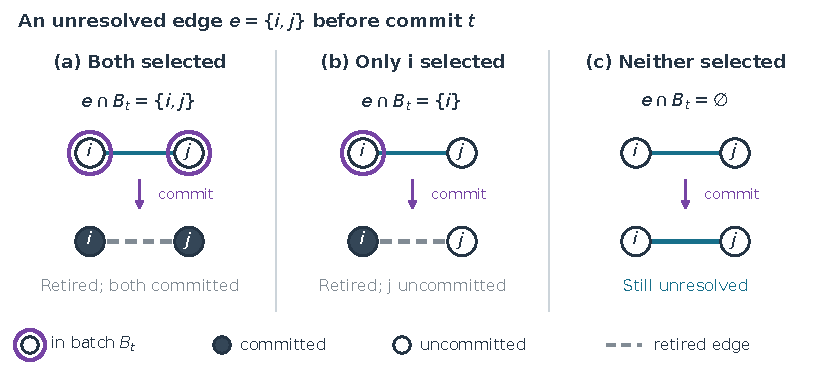
\includegraphics[width=\linewidth]{figures/c45_readability_2026-09-22/output/pdf/commit_cases.pdf}
 \caption{Three possible batch selections on an initially unresolved edge.
 Each panel shows the edge before (top) and after (bottom) one commit.
 Purple rings mark membership in $B_t$; filled nodes are committed.
 Selecting both endpoints gives a collision; selecting one gives a crossing
 edge. Both events retire the whole edge, but in (b) $j$ remains uncommitted.
 Selecting neither endpoint leaves the edge unresolved. The proof records
 the edge identity and both triggers in (a)--(b); the target matching itself
 is unchanged.}
 \label{fig:c4-matching-states}
\end{figure}


% Please keep this introduction with the first component-law definitions.
\Needspace{7\baselineskip}
\emph{Factor the two batch laws.}
Fix a compatible instance \(I\) and visible history \(h\), and write
\(B_t=B_t(h)\). Recall the committed set \(G(h)\), its values \(x_{G(h)}\),
and commit state \(y_t(h)\) from \cref{app:lower-proof-midpoint}.
For each edge \(e\in\HiddenMatching\), define two masses on
\(\Vocab^{e\cap B_t}\):
\begin{align*}
 p_e(z_{e\cap B_t})
 &:=\HardEdgeLaw{e}{I}\!\left(
   X_{e\cap B_t}=z_{e\cap B_t}
   \,\middle|\,
   X_{e\cap G(h)}=x_{e\cap G(h)}
 \right),\\
 \widehat p_e(z_{e\cap B_t})
 &:=\prod_{j\in e\cap B_t}
       \HardOracleRowMass{I}{y_t(h)}{j}{z_j}.
\end{align*}
The first is a conditional mass. The second is normalized because its
coordinates are distinct:
\[
 \sum_{z_{e\cap B_t}}p_e(z_{e\cap B_t})=1,
 \qquad
 \sum_{z_{e\cap B_t}}\widehat p_e(z_{e\cap B_t})
 =\prod_{j\in e\cap B_t}
   \left[\sum_{z_j\in\Vocab}
          \HardOracleRowMass{I}{y_t(h)}{j}{z_j}\right]=1.
\]
If \(e\cap B_t=\varnothing\), the space has one empty assignment and
both masses equal one there.

The sets \(e\cap B_t\) partition \(B_t\).
The edgewise product target law and the oracle product rule give
\begin{align*}
 \HardExactBatchLaw{t}{I}(z\mid h)
 &=\frac{\displaystyle\prod_{e\in\HiddenMatching}
      \HardEdgeLaw{e}{I}
       (X_{e\cap B_t}=z_{e\cap B_t},\,
        X_{e\cap G(h)}=x_{e\cap G(h)})}
     {\displaystyle\prod_{e\in\HiddenMatching}
      \HardEdgeLaw{e}{I}
       (X_{e\cap G(h)}=x_{e\cap G(h)})}\\
 &=\prod_{e\in\HiddenMatching}p_e(z_{e\cap B_t}),\\
 \HardProductBatchLaw{t}{I}(z\mid h)
 &=\prod_{j\in B_t}\HardOracleRowMass{I}{y_t(h)}{j}{z_j}
 =\prod_{e\in\HiddenMatching}\widehat p_e(z_{e\cap B_t}).
\end{align*}
Strict positivity makes every conditioning denominator positive.
These are products at fixed \(I,h\), before averaging over the instance.
Consequently,
\begin{equation}
 \sqrt{\HardExactBatchLaw{t}{I}(z\mid h)
       \HardProductBatchLaw{t}{I}(z\mid h)}
 =\prod_{e\in\HiddenMatching}
       \sqrt{p_e(z_{e\cap B_t})\widehat p_e(z_{e\cap B_t})}.
 \label{app:eq:commit-midpoint-numerator-factorization}
\end{equation}

\emph{Normalize edge by edge.}
Summing the preceding product over the disjoint coordinate blocks gives
\begin{align}
 \HardLocalAffinity{t}{I,h}
 &=\sum_{z\in\Vocab^{B_t}}
     \prod_{e\in\HiddenMatching}
       \sqrt{p_e(z_{e\cap B_t})\widehat p_e(z_{e\cap B_t})}\notag\\
 &=\prod_{e\in\HiddenMatching}
     \left[\sum_{u\in\Vocab^{e\cap B_t}}
                 \sqrt{p_e(u)\widehat p_e(u)}\right]\notag\\
 &=\prod_{e\in\HiddenMatching}\HellingerAffinity(p_e,\widehat p_e).
 \label{app:eq:local-affinity-survivor-factorization}
\end{align}
This is the product-affinity identity of
\cref{app:lem:finite-hellinger-calculus}, with index set
\(J=\HiddenMatching\), spaces \(\mathcal X_e=\Vocab^{e\cap B_t}\),
and the two component masses defined above.
Dividing the numerator product by this positive normalizing product yields
\begin{equation}
 \HardMidpointKernel{t}{I}(z\mid h)
 =\prod_{e\in\HiddenMatching}
 \frac{\sqrt{p_e(z_{e\cap B_t})\widehat p_e(z_{e\cap B_t})}}
      {\displaystyle\sum_{u\in\Vocab^{e\cap B_t}}
                 \sqrt{p_e(u)\widehat p_e(u)}}.
 \label{app:eq:normalized-commit-survivor-likelihood}
\end{equation}
Each factor is normalized: its sum over its coordinate block is its
denominator divided by itself, hence one. On an empty block, both numerator
and denominator are one.

At the fixed observed value \(z\), the factors have the following
dependencies:
\begin{center}
\small
\begin{tabularx}{\linewidth}{@{}>{\raggedright\arraybackslash}p{.23\linewidth}
 >{\raggedright\arraybackslash}X@{}}
\toprule
Edge status & What determines its normalized factor? \\
\midrule
Retired earlier
& Its identity and both triggers, the committed values, and the selected
batch are already in \(\OpAnalyticField{s}\). \\
\addlinespace
Retired in this commit
& Its identity and both triggers are in \(\RetiredRecordValue\);
the remaining inputs are in the current history. \\
\addlinespace
Still unresolved
& It misses \(B_t\), so \(e\cap B_t=\varnothing\) and its factor is \(1\),
for every possible edge identity and trigger assignment. \\
\bottomrule
\end{tabularx}
\end{center}
Thus the normalized kernel is unchanged when the survivor configuration
changes. The exact value of a collision's affinity is needed later in
\cref{app:lem:collision-affinity}; here only this independence is needed.

\emph{Include the oracle replies and identify the support.}
On an unresolved edge, both endpoints are still masked in \(y_t(h)\),
so every commit row there is \(\HardMarginal\).
Rows on earlier retired edges are determined by their recorded identities
and triggers, through \eqref{app:eq:hard-oracle}.
Hence the whole commit-row tuple is fixed by \(\OpAnalyticField{s}\).
For a compatible observation \(o=(\mathbf q,z)\),
\begin{align*}
 \OpSurvivorLikelihood{s}{(\mathbf q,z)}{\SurvivorConfigA}{\RetiredRecordValue}
 &=\mathbf 1\!\left\{
      \mathbf q=(\HardOracleRow{I}{y_t(h)}{j})_{j\in B_t}
    \right\}
    \HardMidpointKernel{t}{I}(z\mid h)\\
 &=\HardMidpointKernel{t}{I}(z\mid h)>0.
\end{align*}
The fixed old and new retirement records, together with
\(\SurvivorConfigA\), specify \(I\). The table shows that the resulting
likelihood has the same positive value for every compatible
\(\SurvivorConfigA\).

Every previously unresolved edge touching \(B_t\) is in
\(\RetiredRecordValue\). Thus
\(\OpUnresolvedVertices{s+1}\cap B_t=\varnothing\), and no surviving
candidate is tested by this commit. The full support is
\[
 \operatorname{PM}(\OpUnresolvedVertices{s+1})
 \times\prod_{i\in\OpUnresolvedVertices{s+1}}\OpRemainingTriggers{i}{s},
 \qquad
 \OpRemainingTriggers{i}{s+1}=\OpRemainingTriggers{i}{s}
 \quad(i\in\OpUnresolvedVertices{s+1}).
\]
Indeed, each configuration in this product extends uniquely with the
retired record, produces the same oracle rows, and assigns positive
midpoint probability to the observed batch value.
It retires exactly the same edges because the surviving vertices
are disjoint from \(B_t\).

\emph{5. Normalize the posterior and conclude (IH\(_{s+1}\)).}
Steps 3--4 give the full support
\[
 \mathcal Z_{s+1}:=
 \operatorname{PM}(\OpUnresolvedVertices{s+1})
 \times\prod_{i\in\OpUnresolvedVertices{s+1}}
                 \OpRemainingTriggers{i}{s+1}.
\]
Step~2 gives equal pre-observation weights, and the query or commit
calculation gives equal positive likelihoods on this support.
Consequently, for any \(\SurvivorConfigA\in\mathcal Z_{s+1}\), the
denominator in \eqref{app:eq:survivor-bayes-odds} is
\begin{align*}
 &\sum_{\mathfrak u\in\mathcal Z_{s+1}}
  \mathbb P(\OpSurvivorState{s+1}=\mathfrak u,
       \OpRetiredRecord{s}=\RetiredRecordValue\mid\OpAnalyticField{s})
       \OpSurvivorLikelihood{s}{o}{\mathfrak u}{\RetiredRecordValue}\\
 &\quad=|\mathcal Z_{s+1}|\,
  \mathbb P(\OpSurvivorState{s+1}=\SurvivorConfigA,
       \OpRetiredRecord{s}=\RetiredRecordValue\mid\OpAnalyticField{s})
       \OpSurvivorLikelihood{s}{o}{\SurvivorConfigA}{\RetiredRecordValue}.
\end{align*}
The common numerator is positive, so cancellation yields
\[
 \mathbb P(\OpSurvivorState{s+1}=\SurvivorConfigA
                 \mid\OpAnalyticField{(s+1)})
 =\frac1{|\mathcal Z_{s+1}|}
 =\frac1{|\operatorname{PM}(\OpUnresolvedVertices{s+1})|}
     \prod_{i\in\OpUnresolvedVertices{s+1}}
       \frac1{|\OpRemainingTriggers{i}{s+1}|}.
\]
This is the independent product required by (IH\(_{s+1}\)).
Induction proves the law at every operation boundary, including the
terminal boundary after the last operation.  There the unresolved set is
empty and the law is the point mass on the empty state.
Finally, the event that operation \(s\) is commit \(t\) is already known
at that operation's starting boundary:
\[
 \{s_t=s\}
 =\left\{\sum_{r<s}\mathbf 1\{A_r\text{ is a commit}\}=t-1,
             \ A_s\text{ is a commit}\right\}
 \in\OpAnalyticField{s}.
\]
Apply (IH\(_s\)) on each of these events to obtain the law at the
adaptive boundary \(s_t\).  At that boundary,
\(\OpSurvivorState{s_t}=\SurvivorState{t}\) and
\(\OpAnalyticField{s_t}=\AnalyticField{t}\), hence
\eqref{app:eq:strong-survivor-invariant} at every pre-commit boundary.
\end{proof}
\fi

% This figure is also used by the subsequent edge-counting argument, so it
% remains compiled even though the legacy proof containing its old call site
% is retained only as noncompiled source.
% Please show each local selection pattern at manuscript width, without a full-page float.
\begin{figure}[!htbp]
 \centering
 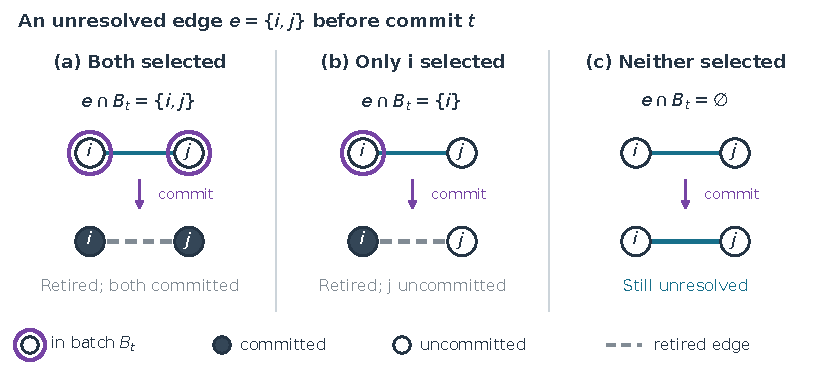
\includegraphics[width=\linewidth]{figures/c45_readability_2026-09-22/output/pdf/commit_cases.pdf}
 \caption{Three possible batch selections on an initially unresolved edge.
 Each panel shows the edge before (top) and after (bottom) one commit.
 Purple rings mark membership in $B_t$; filled nodes are committed.
 Selecting both endpoints gives a collision; selecting one gives a crossing
 edge. Both events retire the whole edge, but in (b) $j$ remains uncommitted.
 Selecting neither endpoint leaves the edge unresolved. The proof records
 the edge identity and both triggers in (a)--(b); the target matching itself
 is unchanged.}
 \label{fig:c4-matching-states}
\end{figure}


\paragraph{One source, at most one candidate per submission.}
Recall from \cref{app:eq:unresolved-matching-update,app:eq:retirement-record}
that the number of query-retired edges is
\[
 \GenieDeletions
 =\sum_{s:\,A_s\text{ is a query}}
   |\OpUnresolvedMatching{s}\setminus\OpUnresolvedMatching{s+1}|.
\]
Commit retirements do not contribute, and simultaneous hits at both endpoints
count as one edge.
A state \(y\) tests at most one candidate \(\HardTest{y}{i}\) at each source
\(i\), regardless of how many returned rows are inspected.
Together with the conditional uniformity in
\cref{app:lem:unresolved-invariant}, this gives the following bound directly.

\begin{lemma}[Equality-test disclosure]
\label{app:lem:query-disclosure}
For any algorithm using at most \(\QueryBudget{}\) counterfactual submissions,
\begin{equation}
 \mathbb E\GenieDeletions\le\frac{N\QueryBudget{}}{\HardBankSize}.
 \label{app:eq:expected-query-deletions}
\end{equation}
\end{lemma}

\begin{proof}
All probabilities and expectations use the joint instance--midpoint law
\eqref{app:eq:joint-instance-midpoint-law}, with the decision-rule seed
\(w\) fixed. The execution below is the midpoint execution.
It suffices to consider integer \(\QueryBudget{}\): for a noninteger
budget, apply the integer result to \(\lfloor\QueryBudget{}\rfloor\),
whose bound is no larger.
If \(\QueryBudget{}=0\), there are no query hits and
\(\GenieDeletions=0\). If \(\QueryBudget{}\ge\HardBankSize\), the bound
follows from \(\GenieDeletions\le N/2\le N\QueryBudget{}/\HardBankSize\).
Hence assume \(1\le\QueryBudget{}<\HardBankSize\).

\emph{1. Bound the hit probability at one query.}
Fix a vertex \(i\). Number counted counterfactual submissions by
\(k=1,2,\ldots\); commits may occur between them.
The distinguished all-mask preprocessing readout tests no candidate
and is not included in this count.
At the \(k\)-th such query, let \(s\) be its operation index and write
\(y=\OpSubmittedState{s}\), as in \cref{app:eq:operation-action}.
Recall that
\(\OpUnresolvedVertices{s}=\bigcup_{e\in\OpUnresolvedMatching{s}}e\)
is the unresolved vertex set just before this operation
(\cref{app:eq:unresolved-vertices}).
The past and selected action determine whether operation \(s\) is
the \(k\)-th counted query. Thus the operation-boundary conclusion of
\cref{app:lem:unresolved-invariant} applies here even when the query
time and state are chosen adaptively.

If \(i\in\OpUnresolvedVertices{s}\), each of the preceding \(k-1\)
counted submissions has removed at most one candidate at \(i\).
Commits leave the candidate set of a surviving vertex unchanged, by
\cref{app:eq:operation-candidates}. Consequently,
\[
 |\OpRemainingTriggers{i}{s}|
 \ge \HardBankSize-(k-1)=\HardBankSize-k+1.
\]
Conditional on \(\OpAnalyticField{s}\), the submitted state is fixed
and \(\TriggerIndex{i}\) is uniform on
\(\OpRemainingTriggers{i}{s}\). Therefore
\begin{align}
 \mathbb P(\HardHit{y}{i}=1\mid\OpAnalyticField{s})
 &=\mathbb P(\TriggerIndex{i}=\HardTest{y}{i}
                  \mid\OpAnalyticField{s})\notag\\
 &=\frac{\mathbf 1\{\HardTest{y}{i}\in\OpRemainingTriggers{i}{s}\}}
         {|\OpRemainingTriggers{i}{s}|}
 \le\frac1{\HardBankSize-k+1}.
 \label{app:eq:query-conditional-hit-bound}
\end{align}
A mask, background token, or previously excluded candidate gives numerator
zero. If the edge has already retired, there can be no further hit
\emph{while unresolved}, regardless of later oracle replies.

\emph{2. Accumulate the probabilities without assuming independence.}
For \(0\le k\le\QueryBudget{}\), define
\[
 p_{i,k}:=
 \mathbb P\!\left(
 \begin{gathered}
 i\text{ has a query hit while its edge is unresolved}\\
 \text{among the first }k\text{ counted submissions}
 \end{gathered}
 \right),
 \qquad p_{i,0}=0.
\]
If the execution contains fewer than \(k\) counted submissions, this event
uses all those that occurred; no extra queries are executed.
A hit retires the edge, so \(i\) can have at most one hit while unresolved.
The increment \(p_{i,k}-p_{i,k-1}\) is therefore the probability of such
a hit at query \(k\).

To bound this increment, condition on each possible analytic history
just before query \(k\), apply
\eqref{app:eq:query-conditional-hit-bound} when \(i\) is unresolved,
and average over these histories. This gives
\begin{align}
 p_{i,k}-p_{i,k-1}
 &\le
 \frac{\mathbb P(\text{query }k\text{ occurs and }i
                  \text{ is unresolved just before it})}
      {\HardBankSize-k+1}\notag\\
 &\le\frac{1-p_{i,k-1}}{\HardBankSize-k+1}.
 \label{app:eq:query-hit-recurrence}
\end{align}
For the last inequality, an unresolved vertex has not hit earlier.
Earlier retirement by a mate hit or a commit, as well as early termination,
can only remove paths from the event in the numerator.
Simultaneous hits at \(i\) and its mate still count as a hit at \(i\):
the edge was unresolved immediately before that query.

Rearranging \eqref{app:eq:query-hit-recurrence} step by step yields
\begin{align*}
 1-p_{i,k}
 &=1-p_{i,k-1}-(p_{i,k}-p_{i,k-1})\\
 &\ge(1-p_{i,k-1})
       \left(1-\frac1{\HardBankSize-k+1}\right)\\
 &=(1-p_{i,k-1})
       \frac{\HardBankSize-k}{\HardBankSize-k+1}.
\end{align*}
Starting from \(1-p_{i,0}=1\) and applying this inequality successively,
\begin{align*}
 1-p_{i,\QueryBudget{}}
 &\ge
 \prod_{k=1}^{\QueryBudget{}}
       \frac{\HardBankSize-k}{\HardBankSize-k+1}\\
 &=\frac{\HardBankSize-1}{\HardBankSize}
   \frac{\HardBankSize-2}{\HardBankSize-1}\cdots
   \frac{\HardBankSize-\QueryBudget{}}
        {\HardBankSize-\QueryBudget{}+1}\\
 &=\frac{\HardBankSize-\QueryBudget{}}{\HardBankSize}.
\end{align*}
For \(\QueryBudget{}=1\) the product has just its first factor.
The cancellation therefore gives
\begin{equation}
 p_{i,\QueryBudget{}}
 \le 1-\frac{\HardBankSize-\QueryBudget{}}{\HardBankSize}
 =\frac{\QueryBudget{}}{\HardBankSize}.
 \label{app:eq:query-source-hit-bound}
\end{equation}
This multiplication iterates conditional probability bounds; it does not
assume independent queries.

\emph{3. Count retired edges by their successful endpoints.}
At a query, an unresolved edge retires exactly when at least one of its
endpoints hits. For binary bits \(b_u,b_v\),
\(\mathbf 1\{b_u+b_v\ge1\}\le b_u+b_v\); two simultaneous hits still retire
only one edge. Hence, pathwise,
\[
 \begin{aligned}
 \GenieDeletions
 &=\sum_{s:\,A_s\text{ is a query}}
   \sum_{\{u,v\}\in\OpUnresolvedMatching{s}}
   \mathbf 1\{\HardHit{\OpSubmittedState{s}}{u}
              +\HardHit{\OpSubmittedState{s}}{v}\ge1\}\\
 &\le
   \sum_{i=1}^N
   \sum_{\substack{s:\,A_s\text{ is a query}\\
                    i\in\OpUnresolvedVertices{s}}}
             \HardHit{\OpSubmittedState{s}}{i}.
 \end{aligned}
\]
The change from edges to vertices uses that every unresolved vertex lies
on exactly one matching edge.
For each \(i\), the inner sum is either zero or one, because its first
hit retires its edge. It is thus the indicator of the event defining
\(p_{i,\QueryBudget{}}\). Taking expectations and using
\(\mathbb E\mathbf 1_E=\mathbb P(E)\) gives
\[
 \begin{aligned}
 \mathbb E\GenieDeletions
 &\le
 \sum_{i=1}^N\mathbb E\!\left[
   \sum_{\substack{s:\,A_s\text{ is a query}\\
                    i\in\OpUnresolvedVertices{s}}}
             \HardHit{\OpSubmittedState{s}}{i}\right]\\
 &=\sum_{i=1}^N p_{i,\QueryBudget{}}
 \le\sum_{i=1}^N\frac{\QueryBudget{}}{\HardBankSize}
 =\frac{N\QueryBudget{}}{\HardBankSize}.
 \end{aligned}
\]
No independence between vertices is used.
\end{proof}
\FloatBarrier

\subsection{Common collision bookkeeping}
\label{app:lower-proof-collisions}

We count how matching edges leave the unresolved-edge set; this pathwise
identity supplies the batch-size constraint in the collision lower-tail
proof. Recall that \(\UnresolvedVertices{t}\) contains the vertices on
edges still unresolved immediately before commit \(t\), after any preceding
queries. At this boundary, operation \(s_t\), the unresolved edge set is
\(\OpUnresolvedMatching{s_t}\), as in
\cref{app:eq:unresolved-matching-update,app:eq:remaining-trigger-set}.
Put \(\UnresolvedVertexCount{t}:=|\UnresolvedVertices{t}|\).
Removing whole edges makes this number even.

For the selected batch \(B_t\), define its active part and collision count:
\begin{equation}
 \ActiveBatch{t}:=B_t\cap\UnresolvedVertices{t},
 \qquad
 \ActiveBatchSize{t}:=|\ActiveBatch{t}|,
 \qquad
 \CollisionCount{t}:=
 \bigl|\{e\in\OpUnresolvedMatching{s_t}:
               e\subseteq\ActiveBatch{t}\}\bigr|,
 \qquad
 \TotalCollisions:=\sum_t\CollisionCount{t}.
 \label{app:eq:unresolved-batch-and-collisions}
\end{equation}
An unresolved edge has no committed endpoint, so
\(\UnresolvedVertices{t}\subseteq\ResidualPositionsAt{G_{t-1}}\).
The inclusion can be strict: query-retired endpoints and the uncommitted
mate of a commit-retired endpoint remain uncommitted but are no longer
active. Figure~\ref{fig:c4-matching-states}(b) shows the latter case.
A later commit of that mate creates no new unresolved-edge collision.

Let \(\ActiveRoundCount:=|\{t:\ActiveBatchSize{t}\ge1\}|\le\RoundBudget{}\)
be the number of rounds with a nonempty active batch.

\begin{lemma}[Pathwise edge-counting identity]
\label{app:lem:pathwise-edge-counting}
Under the retirement rules in \cref{app:eq:unresolved-matching-update},
every complete execution satisfies the pathwise identity
\begin{equation}
 \frac N2
 =\GenieDeletions+
  \sum_t(\ActiveBatchSize{t}-\CollisionCount{t}).
 \label{app:eq:lower-edge-ledger}
\end{equation}

Consequently,
\begin{equation}
 \sum_{t:\ActiveBatchSize{t}\ge1}
   (\ActiveBatchSize{t}-1)
 =\frac N2-\GenieDeletions+\TotalCollisions-\ActiveRoundCount
 \ge\frac N2-\GenieDeletions-\RoundBudget{}.
 \label{app:eq:active-excess-ledger}
\end{equation}
\end{lemma}

\begin{proof}
An active batch touches exactly
\(\ActiveBatchSize{t}-\CollisionCount{t}\) previously unresolved edges.
Indeed, its \(\CollisionCount{t}\) internal edges use
\(2\CollisionCount{t}\) vertices, while every remaining active vertex lies
on a distinct crossing edge. Thus the number touched is
\[
 \underbrace{\CollisionCount{t}}_{\text{internal edges}}
 +\underbrace{(\ActiveBatchSize{t}-2\CollisionCount{t})}_{\text{crossing edges}}
 =\ActiveBatchSize{t}-\CollisionCount{t}.
\]
Since every position is eventually committed, every original matching
edge is retired exactly once: either at a successful counterfactual
trigger test (query retirement), or at its first active commit batch
(commit retirement). Summing over the \(N/2\) original edges proves
\eqref{app:eq:lower-edge-ledger}.

Finally,
\(\sum_{t:\ActiveBatchSize{t}\ge1}(\ActiveBatchSize{t}-1)
=\sum_t\ActiveBatchSize{t}-\ActiveRoundCount\).
Substituting
\(\sum_t\ActiveBatchSize{t}=N/2-\GenieDeletions+\TotalCollisions\)
from \eqref{app:eq:lower-edge-ledger}, then using
\(\TotalCollisions\ge0\) and \(\ActiveRoundCount\le\RoundBudget{}\),
gives \eqref{app:eq:active-excess-ledger}.
\end{proof}

\subsection{A Laplace bound for uniform-matching collisions}
\label{app:lower-proof-matching-laplace}

The next lemma is a finite combinatorial statement independent of the hard
oracle and the adaptive decision rule. It gives a conditional
Laplace bound used below to derive an adaptive lower-tail estimate.

\paragraph{Intuition.}
For a fixed set of $k$ vertices in a uniform matching on $n$ vertices,
each unordered pair is an edge with probability $1/(n-1)$.  Hence the
expected number of internal edges is
\[
 \binom{k}{2}\frac1{n-1}
 =\frac{k(k-1)}{2(n-1)}
 \simeq\frac{k^2}{n}\qquad(k\ge2).
\]
To obtain a lower-tail estimate rather than only a mean, the proof exposes
order $k$ edges, each with conditional success probability at least order
$k/n$.  Their Laplace factors multiply by successive conditioning; the
exposures need not be independent.

\begin{lemma}[Internal-edge Laplace transform]
\label{app:lem:matching-collision-laplace}
Let \(M\) be a uniformly random perfect matching on a labeled set \(U\) of
even cardinality \(n\ge 2\). Fix \(S\subseteq U\), put \(k:=|S|\), and let
\[
 \InternalEdgeCount{S}:=|\{e\in M:e\subseteq S\}|.
\]
Then, for every \(t>0\),
\begin{equation}
 \mathbb E e^{-t\InternalEdgeCount{S}}
 \le
 \exp\left\{
  -\frac{1-e^{-t}}{32}\frac{\PositivePart{k-1}^2}{n}
 \right\}.
 \label{app:eq:matching-collision-laplace}
\end{equation}
\end{lemma}

\begin{proof}

\emph{1. Handle sets of size at most three.}
For \(k\in\{0,1\}\), both sides of
\eqref{app:eq:matching-collision-laplace} equal one. For
\(k\in\{2,3\}\), two internal matching edges would require four distinct
vertices of \(S\). Thus \(\InternalEdgeCount{S}\in\{0,1\}\), and
\[
 \mathbb E\InternalEdgeCount{S}
 =0\cdot\mathbb P(\InternalEdgeCount{S}=0)
  +1\cdot\mathbb P(\InternalEdgeCount{S}=1)
 =\mathbb P(\InternalEdgeCount{S}=1).
\]
Also, writing the edge count as a sum of indicators and taking expectations,
\begin{equation}
 \mathbb E \InternalEdgeCount{S}
 =\sum_{\{u,v\}\subseteq S}\mathbb P(\{u,v\}\in M)
 =\frac{\binom{k}{2}}{n-1}
 =\frac{k(k-1)}{2(n-1)}.
 \label{app:eq:small-set-internal-edge-mean}
\end{equation}
Writing \(a_t:=1-e^{-t}\in(0,1)\), the same two possible values give
\begin{align*}
 \mathbb E e^{-t\InternalEdgeCount{S}}
 &=\mathbb P(\InternalEdgeCount{S}=0)
   +e^{-t}\mathbb P(\InternalEdgeCount{S}=1)\\
 &=1-(1-e^{-t})\mathbb P(\InternalEdgeCount{S}=1)
 =1-a_t\mathbb E\InternalEdgeCount{S}.
\end{align*}
Using \(1-v\le e^{-v}\) for \(v\ge0\), we obtain
\[
 \mathbb E e^{-t\InternalEdgeCount{S}}
 =1-a_t\mathbb E \InternalEdgeCount{S}
 \le e^{-a_t\mathbb E \InternalEdgeCount{S}}
 \le
 \exp\left\{-\frac{a_t}{32}
                   \frac{(k-1)^2}{n}\right\},
\]
where the last inequality follows directly from
\eqref{app:eq:small-set-internal-edge-mean} for \(k=2,3\).


\emph{2. Expose edges and bound each conditional success probability.}
It remains to consider \(k\ge 4\). Partition \(S=A\sqcup B\) with
\(|A|=\lfloor k/2\rfloor\) and \(|B|=\lceil k/2\rceil\), and put
\(m:=\lfloor k/4\rfloor\). We reveal edges of the original matching
\(M\) on the full set \(U\), not of a matching restricted to \(S\).
Only the starting endpoint is required to lie in \(A\); its mate can lie
in \(A\), \(B\), or \(U\setminus S\).

Fix an ordering of \(U\). Let \(U_0:=U\), and for \(j=1,\ldots,m\) define
\begin{align*}
 a_j&:=\min(A\cap U_{j-1}),
 &b_j&:=\operatorname{mate}_{M}(a_j),\\
 e_j&:=\{a_j,b_j\}\in M,
 &U_j&:=U_{j-1}\setminus\{a_j,b_j\}.
\end{align*}
Thus \(U_{j-1}\) consists of the vertices whose matching edges have not yet
been revealed; these vertices are already matched in \(M\).
The minimum uses the fixed ordering, so the choice of \(a_j\) depends only
on the earlier revealed edges. It is well-defined because each previous
edge removes at most two vertices from \(A\), and
\[
 |A\cap U_{j-1}|
 \ge\lfloor k/2\rfloor-2(j-1)
 \ge2m-2(j-1)
 \ge2>0
 \qquad(1\le j\le m).
\]

Define the success indicator by
\[
 X_j:=\mathbf1_{\{b_j\in B\cap U_{j-1}\}},
 \qquad
 \{X_j=1\}=\{\operatorname{mate}_{M}(a_j)\in B\cap U_{j-1}\}.
\]
Since every starting endpoint \(a_\ell\) lies in \(A\), each previous
edge \(e_\ell\) removes at most one vertex from \(B\). Consequently,
\[
 |B\cap U_{j-1}|
 \ge\lceil k/2\rceil-(j-1)
 \ge k/2-(m-1)
 \ge k/4,
 \qquad
 |U_{j-1}|=n-2(j-1).
\]
Conditional on \(e_1,\ldots,e_{j-1}\), the remaining matching is uniform
on \(U_{j-1}\): every perfect matching there has exactly one extension
by the already revealed edges. Each possible mate of \(a_j\) has the same
number of matching completions, so
\[
 \mathbb P(b_j=v\mid e_1,\ldots,e_{j-1})
 =\frac1{|U_{j-1}|-1}
 \quad\text{for }v\in U_{j-1}\setminus\{a_j\}.
\]
Summing over the allowable mates in \(B\), which never include
\(a_j\in A\), gives
\begin{align*}
 \mathbb P(X_j=1\mid e_1,\ldots,e_{j-1})
 &=\sum_{v\in B\cap U_{j-1}}
   \mathbb P(b_j=v\mid e_1,\ldots,e_{j-1})\\
 &=\frac{|B\cap U_{j-1}|}{|U_{j-1}|-1}
 \ge\frac{k/4}{n}=\frac{k}{4n}.
\end{align*}
The earlier indicators \(X_1,\ldots,X_{j-1}\) are determined by these
revealed edges. Adding them to the conditioning therefore gives the same
probability:
\begin{equation}
 \mathbb P(X_j=1\mid X_1,\ldots,X_{j-1},
               \text{all preceding exposed edges})
 \ge u:=\frac{k}{4n}.
 \label{app:eq:matching-cross-success}
\end{equation}
Removing both endpoints after each exposure makes \(e_1,\ldots,e_m\)
distinct. If \(X_j=1\), then \(a_j\in A\) and \(b_j\in B\), so
\(e_j\subseteq A\cup B=S\). Therefore
\[
 \sum_{j=1}^mX_j
 =|\{e_j:1\le j\le m,\ X_j=1\}|
 \le|\{e\in M:e\subseteq S\}|=\InternalEdgeCount{S}.
\]

\emph{3. Iterate conditional Laplace factors without independence.}
For one exposure, the Bernoulli identity and the preceding probability
bound give
\begin{align*}
 &\mathbb E[e^{-tX_j}\mid\text{preceding exposed edges}]\\
 &\qquad=1-(1-e^{-t})\Pr(X_j=1\mid\text{preceding exposed edges})\\
 &\qquad\le1-u(1-e^{-t}).
\end{align*}
For \(1\le r\le m\), condition on the first \(r-1\) exposed edges.
The earlier factors are measurable with respect to this record, so
\begin{align*}
 \mathbb E e^{-t\sum_{j=1}^{r}X_j}
 &=\mathbb E\!\left[
   e^{-t\sum_{j=1}^{r-1}X_j}
   \mathbb E(e^{-tX_r}\mid\text{first \(r-1\) exposed edges})\right]\\
 &\le[1-u(1-e^{-t})]\,
      \mathbb E e^{-t\sum_{j=1}^{r-1}X_j}.
\end{align*}
Starting with the empty sum at \(r=0\), whose exponential is one, and
iterating to \(r=m\) gives the power below without an independence
assumption:
\begin{align}
 \mathbb E e^{-t\InternalEdgeCount{S}}
 &\le \mathbb E\exp\left\{-t\sum_{j=1}^mX_j\right\}\notag\\
 &\le\{1-u(1-e^{-t})\}^{m}
 \le\exp\{-mu(1-e^{-t})\}.
 \label{app:eq:matching-exposure-laplace}
\end{align}
Since \(m\ge k/8\) for \(k\ge4\),
\(mu\ge k^2/(32n)\ge(k-1)^2/(32n)\). Substitution in
\eqref{app:eq:matching-exposure-laplace} proves
\eqref{app:eq:matching-collision-laplace}.
\end{proof}

\subsection{An adaptive lower tail for batch collisions}
\label{app:lower-proof-collision-tail}

The conditional Laplace bound and the edge-counting identity now force many collisions
with constant probability under the joint instance--midpoint law. This is
the input needed to accumulate edge-level discrepancy nonlinearly; no
independence between commit rounds is assumed. Recall that
\(\TotalCollisions=\sum_t\CollisionCount{t}\) counts the unresolved edges
whose two endpoints are committed in the same active batch, as defined in
\eqref{app:eq:unresolved-batch-and-collisions}.

\paragraph{Intuition.}
If order $N$ unresolved vertices were spread evenly across $\RoundBudget$
batches while the unresolved pool had size order $N$, the collision scale
would be
\[
 \RoundBudget\frac{(N/\RoundBudget)^2}{N}
 =\frac{N}{\RoundBudget}.
\]
The proof does not assume even batches or a fixed pool: the edge-counting identity
forces enough total active batch mass, Cauchy--Schwarz gives the same
$N/\RoundBudget$ scale, and the conditional Laplace bound turns that
pathwise mass into a constant-probability collision event.

\begin{proposition}[Adaptive collision lower tail]
\label{app:prop:collision-lower-tail}
Fix a decision-rule seed under the joint law
\eqref{app:eq:joint-instance-midpoint-law}. If
\(\QueryBudget{}\le \HardBankSize/8\) and \(1\le \RoundBudget{}\le N/8\), then
\begin{equation}
 \mathbb P\left(
   \TotalCollisions\ge\frac{N}{8192\RoundBudget{}}
 \right)
 \ge
 \frac12-\exp\left\{-\frac{N}{8192\RoundBudget{}}\right\}.
 \label{app:eq:collision-lower-tail}
\end{equation}
In particular, if \(\RoundBudget{}\le N/16384\), then
\begin{equation}
 \mathbb P\left(
   \TotalCollisions\ge\frac{N}{8192\RoundBudget{}}
 \right)\ge\frac14.
 \label{app:eq:collision-quarter-probability}
\end{equation}
\end{proposition}

\begin{proof}

\emph{1. Fix the pre-exposure information and conditional Laplace bound.}
For an actual commit round \(t\), let \(B_t\) be the batch selected by the
seed-fixed decision rule. Recall the existing notation:
\[
 \ActiveBatch{t}=B_t\cap\UnresolvedVertices{t},
 \qquad
 \UnresolvedVertexCount{t}=|\UnresolvedVertices{t}|,
 \qquad
 \ActiveBatchSize{t}=|\ActiveBatch{t}|,
\]
\[
 \CollisionCount{t}
 =|\{e\in\OpUnresolvedMatching{s_t}:
                    e\subseteq\ActiveBatch{t}\}|,
 \qquad
 \TotalCollisions=\sum_t\CollisionCount{t}.
\]
Thus \(B_t\) is the full commit batch, whereas \(\ActiveBatch{t}\)
contains only its currently unresolved vertices.

After termination, append empty rounds until the total number of indexed
rounds is \(\RoundBudget{}\). In every appended round set
\(B_t=\ActiveBatch{t}=\UnresolvedVertices{t}=\varnothing\), so
\(\UnresolvedVertexCount{t}=\ActiveBatchSize{t}=\CollisionCount{t}=0\).
These rounds add no collision, and hence
\(\TotalCollisions=\sum_{t=1}^{\RoundBudget{}}\CollisionCount{t}\).
Introduce only the following additional abbreviation:
\[
 A_t:=
 \begin{cases}
  \PositivePart{\ActiveBatchSize{t}-1}^2/\UnresolvedVertexCount{t},
      &\UnresolvedVertexCount{t}>0,\\
  0,&\UnresolvedVertexCount{t}=0.
 \end{cases}
\]
The pre-commit analytic field \(\AnalyticField{t}\) determines both the
selected batch \(B_t\) and the unresolved set \(\UnresolvedVertices{t}\),
hence also \(\ActiveBatch{t}=B_t\cap\UnresolvedVertices{t}\).
Selecting \(B_t\) adds no observation: the matching edges incident to
\(\ActiveBatch{t}\) and the midpoint values \(X_{B_t}\) have not yet been
exposed. Thus \(\UnresolvedVertexCount{t}\), \(\ActiveBatchSize{t}\),
\(A_t\), and all quantities from earlier rounds are
\(\AnalyticField{t}\)-measurable. For appended empty rounds, use the terminal
field.

By \cref{app:lem:unresolved-invariant}, conditional on \(\AnalyticField{t}\),
the matching on \(\UnresolvedVertices{t}\) is uniform. For
\(\UnresolvedVertexCount{t}\ge2\), apply
\cref{app:lem:matching-collision-laplace} with
\(U=\UnresolvedVertices{t}\), \(S=\ActiveBatch{t}\),
\(n=\UnresolvedVertexCount{t}\), \(k=\ActiveBatchSize{t}\), and Laplace
parameter one. Since \(1-e^{-1}\ge1/2\), this gives
\begin{equation}
 \mathbb E\!\left[e^{-\CollisionCount{t}}\mid\AnalyticField{t}\right]
 \le
 \exp\left\{-\frac{1-e^{-1}}{32}A_t\right\}
 \le e^{-A_t/64}.
 \label{app:eq:conditional-collision-laplace}
\end{equation}
The unresolved set has even cardinality, so
\(\UnresolvedVertexCount{t}=1\) cannot occur. If
\(\UnresolvedVertexCount{t}=0\), then
\(\ActiveBatchSize{t}=\CollisionCount{t}=A_t=0\), and the same display holds
with equality.


\emph{2. Iterate the exponential expectation bound.}
Let \(r=0,\ldots,\RoundBudget{}\) count completed commit rounds, not
individual operations.  Define
\begin{equation}
 \CollisionExponential{r}:=
 \exp\left\{
   -\sum_{t=1}^{r}\CollisionCount{t}
   +\frac1{64}\sum_{t=1}^{r}A_t
 \right\},
 \qquad \CollisionExponential{0}:=1.
 \label{app:eq:collision-supermartingale}
\end{equation}
Both \(\CollisionExponential{r-1}\) and \(A_r\) are measurable with respect
to \(\AnalyticField{r}\), the field immediately before commit \(r\)
after any intervening counterfactual operations. Hence
\eqref{app:eq:conditional-collision-laplace} and the tower property give
\[
 \mathbb E \CollisionExponential{r}
 =
 \mathbb E\!\left[
   \CollisionExponential{r-1}e^{A_r/64}
   \mathbb E(e^{-\CollisionCount{r}}\mid\AnalyticField{r})
 \right]
 \le \mathbb E \CollisionExponential{r-1}.
\]
Iteration yields
\begin{equation}
 \mathbb E \CollisionExponential{\RoundBudget}\le1.
 \label{app:eq:terminal-collision-supermartingale}
\end{equation}
This is the only concentration step; adaptivity is absorbed into the
successive conditional expectations.


\emph{3. Turn edge counting into a pathwise Laplace budget.}
By \cref{app:lem:query-disclosure} and
\(\QueryBudget{}\le\HardBankSize/8\),
\[
 \mathbb E\GenieDeletions
 \le\frac{N\QueryBudget{}}{\HardBankSize}
 \le\frac{N(\HardBankSize/8)}{\HardBankSize}
 =\frac N8.
\]
Because \(\GenieDeletions\ge0\), Markov's inequality gives
\[
 \mathbb P(\GenieDeletions>N/4)
 \le\frac{\mathbb E\GenieDeletions}{N/4}
 \le\frac{N/8}{N/4}=\frac12.
\]
Taking the complement,
\(\mathbb P(\GenieDeletions\le N/4)=1-\mathbb P(\GenieDeletions>N/4)\),
therefore yields
\begin{equation}
 \mathbb P(\GenieDeletions\le N/4)\ge\frac12.
 \label{app:eq:few-genie-deletions-event}
\end{equation}
On this event, the pathwise counting identity
\eqref{app:eq:active-excess-ledger} in \cref{app:lem:pathwise-edge-counting}, the bounds
\(\ActiveRoundCount\le \RoundBudget{}\le N/8\), and
\(\TotalCollisions\ge0\) imply
\begin{equation}
 \sum_{t=1}^{\RoundBudget{}}\PositivePart{\ActiveBatchSize{t}-1}
 \ge \frac N2-\GenieDeletions-\RoundBudget{}
 \ge\frac N8.
 \label{app:eq:pathwise-active-excess}
\end{equation}
Since \(\UnresolvedVertexCount{t}\le N\), the definition of \(A_t\)
implies \(A_t\ge\PositivePart{\ActiveBatchSize{t}-1}^2/N\).
This also holds when \(\UnresolvedVertexCount{t}=0\), because then both
sides are zero. Cauchy--Schwarz over the \(\RoundBudget{}\) indexed rounds
(including appended empty rounds) now gives
\begin{align}
 \sum_{t=1}^{\RoundBudget{}}A_t
 &\ge\frac1N\sum_{t=1}^{\RoundBudget{}}\PositivePart{\ActiveBatchSize{t}-1}^2\notag\\
 &\ge\frac1{N\RoundBudget{}}
       \left(\sum_{t=1}^{\RoundBudget{}}\PositivePart{\ActiveBatchSize{t}-1}\right)^2
 \ge\frac{N}{64\RoundBudget{}}.
 \label{app:eq:pathwise-laplace-budget}
\end{align}


\emph{4. Subtract the small-collision event.}
Set \(x:=N/(8192\RoundBudget{})\). On the intersection
\(\{\GenieDeletions\le N/4\}\cap\{\TotalCollisions<x\}\),
\eqref{app:eq:pathwise-laplace-budget} yields
\[
 \log \CollisionExponential{\RoundBudget}
 =-\TotalCollisions+\frac1{64}\sum_{t=1}^{\RoundBudget{}}A_t
 >-x+\frac{N}{4096\RoundBudget{}}
 =x.
\]
Using \eqref{app:eq:terminal-collision-supermartingale} and Markov's
inequality,
\begin{align*}
 \mathbb P(\GenieDeletions\le N/4,\ \TotalCollisions<x)
 &\le \mathbb P(\CollisionExponential{\RoundBudget}>e^x)\\
 &\le\frac{\mathbb E\CollisionExponential{\RoundBudget}}{e^x}
 \le\frac1{e^x}=e^{-x}.
\end{align*}
Combining with \eqref{app:eq:few-genie-deletions-event},
\begin{align*}
 \mathbb P(\TotalCollisions\ge x)
 &\ge \mathbb P(\GenieDeletions\le N/4,\ \TotalCollisions\ge x)\\
 &=\mathbb P(\GenieDeletions\le N/4)
   -\mathbb P(\GenieDeletions\le N/4,\ \TotalCollisions<x)\\
 &\ge \frac12-e^{-x},
\end{align*}
which proves \eqref{app:eq:collision-lower-tail}.
If \(\RoundBudget{}\le N/16384\), then \(x\ge2\)
and \(1/2-e^{-2}>1/4\), proving
\eqref{app:eq:collision-quarter-probability}.
\end{proof}

\subsection{Collision-affinity bound}
\label{app:lower-proof-affinity}

We combine the midpoint identity with the one-edge Hellinger loss to
convert unresolved collisions into a multiplicative affinity penalty.
Recall our normalization: for probability masses \(p,q\) on the same
finite set \(\mathcal X\),
\(\HellingerAffinity(p,q):=\sum_{x\in\mathcal X}\sqrt{p(x)q(x)}\).
The squared Hellinger distance is
\(\sqHellinger(p,q):=\tfrac12\sum_{x\in\mathcal X}
(\sqrt{p(x)}-\sqrt{q(x)})^2=1-\HellingerAffinity(p,q)\).

\paragraph{Intuition.}
Each unresolved edge whose endpoints are committed together contributes
the factor $1-\HardEdgeDistance$.  Since
$\HardEdgeDistance\simeq\EdgeCoupling^2$,
\[
 1-(1-\HardEdgeDistance)^{\TotalCollisions}
 \simeq
 \min\{1,\EdgeCoupling^2\TotalCollisions\}.
\]
For justification, $1-(1-d)^z\le\min\{1,zd\}$ for integer $z\ge0$, while
$1-(1-d)^z\ge1-e^{-zd}\ge(1-e^{-1})\min\{1,zd\}$.
This is an edge-penalty scale; the next lemma places its expectation below
the actual squared-Hellinger risk.

\begin{lemma}[Affinity loss from unresolved collisions]
\label{app:lem:collision-affinity}
For every fixed decision-rule seed \(w\),
\begin{equation}
 \mathbb E_{I\sim\HardInstancePrior}
 \sqHellinger(\HardTargetLaw{I},\HardOutputLaw{I}{w})
 \ge
 \mathbb E_{I,H}
 \left[1-(1-\HardEdgeDistance)^{\TotalCollisions}\right],
 \label{app:eq:global-collision-affinity}
\end{equation}
where the expectation on the right is under
\eqref{app:eq:joint-instance-midpoint-law}.
\end{lemma}

\begin{proof}
\emph{1. Specify the edge components at a fixed history.}
Fix \(I,w\) and a reachable pre-commit history \(h\), and write
\(B_t=B_t(h)\). As in Step~4 of \cref{app:lem:unresolved-invariant}, the
two component laws on \(\Vocab^{e\cap B_t}\), for
\(e\in\HiddenMatching\), are
\begin{align*}
 p_e(z_{e\cap B_t})
 &:=\HardEdgeLaw{e}{I}
        (z_{e\cap B_t}\mid x_{e\cap G(h)}),\\
 \widehat p_e(z_{e\cap B_t})
 &:=\prod_{j\in e\cap B_t}
       \HardOracleRowMass{I}{y_t(h)}{j}{z_j}.
\end{align*}
The first line is the conditional probability of the current edge
coordinates given the already committed coordinates of that edge.
Both masses sum to one; on an empty coordinate set both equal one on the
empty assignment. The conditional product calculation in that step gives
\[
 \HardExactBatchLaw{t}{I}(z\mid h)
   =\prod_{e\in\HiddenMatching}p_e(z_{e\cap B_t}),
 \qquad
 \HardProductBatchLaw{t}{I}(z\mid h)
   =\prod_{e\in\HiddenMatching}\widehat p_e(z_{e\cap B_t}).
\]
These products are at fixed \(I,h\); each component is a block of batch
coordinates from one edge, not necessarily a single vertex.

\emph{2. Compute the factor of an unresolved collision.}
Partition the unresolved edges according to the number of selected endpoints:
\begin{equation}
 \mathcal E_t^{(r)}:=
 \{e\in\OpUnresolvedMatching{s_t}:
       |e\cap\ActiveBatch{t}|=r\},
 \qquad r\in\{0,1,2\}.
 \label{app:eq:commit-edge-partition}
\end{equation}
Thus the collision-edge set and its size are
\[
 \mathcal E_t^{(2)}
 =\{e\in\OpUnresolvedMatching{s_t}:
                       e\subseteq\ActiveBatch{t}\},
 \qquad
 |\mathcal E_t^{(2)}|=\CollisionCount{t},
 \qquad
 \ActiveBatch{t}=B_t\cap\UnresolvedVertices{t}.
\]
For \(e=\{i,j\}\in\mathcal E_t^{(2)}\), both endpoints belong to \(B_t\)
and neither belongs to \(G(h)\). Thus the exact component has no
conditioning within \(e\), while both oracle rows see their mate masked:
\[
 p_e(z_i,z_j)=\HardEdgeLaw{e}{I}(z_i,z_j),
 \qquad
 \widehat p_e(z_i,z_j)
 =\HardMarginal(z_i)\HardMarginal(z_j)
 =\HardIndependentEdgeLaw{e}(z_i,z_j).
\]
Here the oracle equality uses \eqref{app:eq:hard-oracle}, and the absence
of conditioning from other edges uses the target's edgewise product law.
Consequently,
\(\HellingerAffinity(p_e,\widehat p_e)
 =1-\sqHellinger(\HardEdgeLaw{e}{I},\HardIndependentEdgeLaw{e})
 =1-\HardEdgeDistance\), where \(\HardEdgeDistance\) is defined in
\eqref{app:eq:hard-edge-distance}. In terms of the actual edge masses,
this is
\begin{equation}
 \sum_{z_i,z_j}
 \sqrt{\HardEdgeLaw{e}{I}(z_i,z_j)
       \HardIndependentEdgeLaw{e}(z_i,z_j)}
 =1-\HardEdgeDistance.
 \label{app:eq:one-collision-affinity}
\end{equation}
\emph{3. Bound every remaining component and apply product affinity.}
Since \(p_e\) and \(\widehat p_e\) are probability masses,
\(0\le\HellingerAffinity(p_e,\widehat p_e)\le1\) by Cauchy--Schwarz.
This covers all noncollision components, including previously retired
edges where the oracle need not be exact. More specifically, an unresolved
crossing edge has \(p_e=\widehat p_e=\HardMarginal\), and an edge with
\(e\cap B_t=\varnothing\) has both masses equal to one on the empty
assignment; these components have affinity exactly one.

Apply \cref{app:lem:finite-hellinger-calculus} with index set
\(J=\HiddenMatching\), spaces \(\mathcal X_e=\Vocab^{e\cap B_t}\),
and component laws \(p_e,\widehat p_e\).
The two product laws to which it applies are exactly
\(\HardExactBatchLaw{t}{I}(\cdot\mid h)\) and
\(\HardProductBatchLaw{t}{I}(\cdot\mid h)\) from Step~1.
By the definition \eqref{app:eq:hard-local-affinity} and that lemma,
\begin{align*}
 \HardLocalAffinity{t}{I,h}
 &=\HellingerAffinity\!\left(
      \HardExactBatchLaw{t}{I}(\cdot\mid h),
      \HardProductBatchLaw{t}{I}(\cdot\mid h)\right)\\
 &=\prod_{e\in\HiddenMatching}\HellingerAffinity(p_e,\widehat p_e)\\
 &=\left(\prod_{e\in\mathcal E_t^{(2)}}(1-\HardEdgeDistance)\right)
   \left(\prod_{e\in\HiddenMatching\setminus\mathcal E_t^{(2)}}
                \HellingerAffinity(p_e,\widehat p_e)\right)\\
 &=(1-\HardEdgeDistance)^{\CollisionCount{t}}
   \prod_{e\in\HiddenMatching\setminus\mathcal E_t^{(2)}}
                \HellingerAffinity(p_e,\widehat p_e).
\end{align*}
Every factor in the remaining product lies in \([0,1]\), so
\begin{equation}
 \HardLocalAffinity{t}{I,h}
 \le(1-\HardEdgeDistance)^{\CollisionCount{t}}.
 \label{app:eq:local-collision-affinity}
\end{equation}
\emph{4. Multiply along the adaptive path and average.}
The preceding bound holds at each reached history, including histories
under the midpoint law. Multiplying over rounds and using
\(\TotalCollisions=\sum_t\CollisionCount{t}\) yields
\[
 \prod_t\HardLocalAffinity{t}{I,H_{t-1}}
 \le(1-\HardEdgeDistance)^{\TotalCollisions}.
\]
Using the adaptive identity \eqref{app:eq:adaptive-midpoint-identity}
first at fixed \(I,w\) and then averaging over \(I\) gives
\begin{align*}
 &\mathbb E_I\sqHellinger(\HardTargetLaw{I},\HardOutputLaw{I}{w})\\
 &\quad=1-\mathbb E_I
    \mathbb E_{H\sim\HardMidpointLaw{I}{w}}
       \prod_t\HardLocalAffinity{t}{I,H_{t-1}}\\
 &\quad\ge1-\mathbb E_{I,H}(1-\HardEdgeDistance)^{\TotalCollisions}\\
 &\quad=\mathbb E_{I,H}
       [1-(1-\HardEdgeDistance)^{\TotalCollisions}],
\end{align*}
where the joint expectation uses the conditional midpoint law given \(I,w\).
This proves \eqref{app:eq:global-collision-affinity}.
\end{proof}

\subsection{Nonlinear finite minimax bound}
\label{app:lower-proof-nonlinear}

\paragraph{Intuition.}
When the query budget is a small enough fraction of the bank size,
the preceding two results give
\[
 \text{risk}\ \gtrsim\
 1-\exp\{-cN\EdgeCoupling^2/\RoundBudget\}
 \simeq\min\{1,N\EdgeCoupling^2/\RoundBudget\},
\]
where $c>0$ is a fixed numerical constant.
The constant-probability collision event supplies order
$N/\RoundBudget$ missed edges; each contributes order $\EdgeCoupling^2$.
For a small target tolerance $\varepsilon$, this forces
$\RoundBudget\gtrsim N\EdgeCoupling^2/\varepsilon$.
The proof retains the finite constants and checks the prior-to-minimax
step explicitly.

\begin{proof}[Proof of \cref{app:thm:nonlinear-finite-lower}]

\emph{1. Obtain the nonlinear bound at a fixed seed.}
Fix an arbitrary algorithm in \(\HardAlgorithmClass{\QueryBudget{}}{\RoundBudget{}}\) and a decision-rule
seed \(w\). Suppose \(\QueryBudget{}\le\HardBankSize/8\) and
\(1\le \RoundBudget{}\le N/16384\). By
\cref{app:lem:collision-affinity,app:prop:collision-lower-tail},
\begin{align}
 &\mathbb E_{I\sim\HardInstancePrior}
 \sqHellinger(\HardTargetLaw{I},\HardOutputLaw{I}{w})\notag\\
 &\quad\ge
 \mathbb E_{I,H}
 \left[1-(1-\HardEdgeDistance)^{\TotalCollisions}\right]\notag\\
 &\quad\ge
 \frac14\left[
  1-(1-\HardEdgeDistance)^{N/(8192\RoundBudget{})}
 \right].
 \label{app:eq:nonlinear-fixed-seed-step}
\end{align}
The exponent in the last display need not be an integer: on the event
\(\TotalCollisions\ge N/(8192\RoundBudget{})\), monotonicity of
\(c\mapsto1-(1-\HardEdgeDistance)^c\) gives the displayed lower bound.
Using \(1-d\le e^{-d}\) for \(d\in[0,1]\) and the one-edge estimate
\(\HardEdgeDistance\ge\EdgeCoupling^2/12\) from
\eqref{app:eq:hard-edge-distance}, we obtain
\begin{equation}
 \mathbb E_{I\sim\HardInstancePrior}
 \sqHellinger(\HardTargetLaw{I},\HardOutputLaw{I}{w})
 \ge
 \frac14\left[
  1-\exp\left\{-\frac{N\EdgeCoupling^2}{98304\RoundBudget{}}\right\}
 \right].
 \label{app:eq:nonlinear-fixed-seed-lower}
\end{equation}


\emph{2. Average over seeds and pass from the prior to minimax risk.}
Finally, \(\dTV\ge\sqHellinger\) by
\cref{app:lem:finite-hellinger-calculus}. The decision-rule seed \(W\) is
independent of \(I\sim\HardInstancePrior\), so Tonelli's theorem gives
\begin{align}
 \mathbb E_I\SeedRisk(\mathcal A;\HardTargetLaw{I},\HardOracle{I})
 &=\mathbb E_W\mathbb E_I
    \dTV(\HardTargetLaw{I},\HardOutputLaw{I}{W})\notag\\
 &\ge\mathbb E_W\mathbb E_I
    \sqHellinger(\HardTargetLaw{I},\HardOutputLaw{I}{W})\notag\\
 &\ge\frac14\left[
  1-\exp\left\{-\frac{N\EdgeCoupling^2}{98304\RoundBudget{}}\right\}
 \right].
 \label{app:eq:prior-to-seed-risk}
\end{align}
At least one fixed instance has seed-averaged TV risk at least this
prior average. Taking the supremum over the hard family and then the
infimum over \(\HardAlgorithmClass{\QueryBudget{}}{\RoundBudget{}}\)
proves \eqref{app:eq:nonlinear-finite-lower}.
\end{proof}

\begin{proof}[Proof of
\cref{app:cor:nonlinear-finite-target-tradeoff}]
Suppose the first two alternatives in
\eqref{app:eq:nonlinear-finite-target-alternative} fail. Then
\cref{app:thm:nonlinear-finite-lower} and
\eqref{app:eq:finite-target-risk} imply
\[
 \varepsilon
 \ge
 \frac14\left[
  1-\exp\left\{-\frac{N\EdgeCoupling^2}{98304\RoundBudget{}}\right\}
 \right].
\]
Since \(\varepsilon\le1/8\), rearrangement gives
\begin{align*}
 \frac{N\EdgeCoupling^2}{98304\RoundBudget{}}
 &\le-\log(1-4\varepsilon)\\
 &\le\frac{4\varepsilon}{1-4\varepsilon}
 \le8\varepsilon.
\end{align*}
Here \(-\log(1-u)\le u/(1-u)\) for \(u\in[0,1)\), obtained by integrating
\((1-x)^{-1}\le(1-u)^{-1}\) over \(x\in[0,u]\). Thus
\[
 \RoundBudget{}\ge\frac{N\EdgeCoupling^2}{786432\varepsilon},
\]
which is the third alternative in
\eqref{app:eq:nonlinear-finite-target-alternative}.
\end{proof}

